\documentclass[11pt,oneside]{book}
\usepackage{natbib}
\usepackage{color}
\usepackage{amsmath}
\usepackage{amssymb}
\usepackage{graphicx}
\usepackage{epsfig}
\usepackage{amsmath}
\usepackage{amssymb}
\usepackage{shadow}
\usepackage{tablefootnote}
\usepackage{tabto}
\usepackage{tikz}
\usepackage{graphicx,wrapfig,lipsum}
\usepackage{caption}
\usepackage{subcaption}
\usepackage{esvect}
\usepackage{hyperref}
\usepackage{booktabs}
\usepackage{Myfullpage}
\usepackage{placeins}
%\usepackage{fullname}
\usepackage{times}
\usepackage{covington}
%\usepackage{mathbbol}
\usepackage{amsthm}
\usepackage{amssymb}
\usepackage{url}

%\usepackage{txfonts}
\usepackage{%
  pstricks,
  pst-node}
\usepackage{fancyhdr}
\usepackage{amssymb,amsmath}
\usepackage{epsfig,graphics}
\usepackage{llncsdoc}
\usepackage{enumerate}
\usepackage{amsmath}
\usepackage{algorithm,algorithmic}
\renewcommand{\algorithmicrequire}{\textbf{Inputs:}}
\renewcommand{\algorithmicensure}{\textbf{Outputs:}}

% PSTricks settings and definitions
\let\Oldsection\section
\renewcommand{\section}{\FloatBarrier\Oldsection}

\let\Oldsubsection\subsection
\renewcommand{\subsection}{\FloatBarrier\Oldsubsection}

\let\Oldsubsubsection\subsubsection
\renewcommand{\subsubsection}{\FloatBarrier\Oldsubsubsection}

\psset{nodesep=3pt}
% a state of an automaton
\newcommand{\state}[2]{\circlenode{#1}{#2}}
% an initial state: shaded circle
\newcommand{\istate}[2]{\circlenode[fillstyle=solid,fillcolor=lightgray]{#1}{#2}}
% a final state: double circles with a small separating distance
\newcommand{\fstate}[2]{\circlenode[framesep=0pt]{#1}{\pscirclebox[framesep=1pt]{#2}}}
% an initial and final state
\newcommand{\ifstate}[2]{\circlenode[framesep=0pt]{#1}{\pscirclebox[fillstyle=solid,fillcolor=lightgray,framesep=1pt]{#2}}}
% an arc. parameters:
% 1 (optional): 2 angles
% 2: source node; 3: target node; 4: label.
\newcommand{\trans}[4][angleA=0,angleB=180]{\nccurve[#1]{->}{#2}{#3}\Aput{#4}}
\newcommand{\transdash}[4][angleA=0,angleB=180,linestyle=dashed]{\nccurve[#1]{->}{#2}{#3}\Aput{#4}}
\newcommand{\transdot}[4][angleA=0,angleB=180,linestyle=dotted]{\nccurve[#1]{->}{#2}{#3}\Aput{#4}}
\renewcommand{\baselinestretch}{1.67}
\newcommand{\minispace}{\mbox{\hspace{1mm}}}
\newcommand{\smallspace}{\mbox{\hspace{3mm}}}
\newcommand{\bigspace}{\mbox{\hspace{10mm}}}
\newcommand{\textnl}{\textsl}
\newcommand{\naturals}{\mathbb{N}}
\newtheorem{definition}{Definition}[chapter]
\newtheorem{proposition}{Proposition}[chapter]
\newtheorem{lemma}{Lemma}[chapter]
\newtheorem{exa}{Example}[chapter]
\newtheorem{observation}{Observation}[chapter]
\newtheorem{claim}{Claim}[chapter]
\newtheorem{corollary}{Corollary}[chapter]
\newtheorem{theorem}{Theorem}[chapter]
\newcommand{\comment}[1]{}

\def\ignore#1{}

\begin{document}
\date{\today\\v1.3}
\title{\Huge{The ecology of Web browser}
                \huge
             \\[10mm] Sela Ferdman
             \\[25mm] \Large THESIS SUBMITTED IN PARTIAL FULFILLMENT OF THE
             \\       REQUIREMENTS FOR THE MASTER DEGREE
             \\[15mm] University of Haifa
             \\       Faculty of Social Sciences
             \\       Department of Computer Sciences
             \\[10mm] March, 2015
}
\date{\today\\v1.3}
\maketitle{}

\pagestyle{plain}
\pagenumbering{Roman}

\begin{center}
\Huge
     The ecology of Web browser
\huge
\\[10mm] By: Sela Ferdman
\\[3mm] Supervised By: Dr. Einat Minkov and Dr. Ron Bekkerman
\Large
\\ [10mm]THESIS SUBMITTED IN PARTIAL FULFILLMENT OF THE
\\ REQUIREMENTS FOR THE MASTER DEGREE
\\ [10mm]University of Haifa
\\ [1mm]Faculty of Social Sciences
\\ [1mm]Department of Computer Sciences
\\ [3mm]March, 2015
\\ [8mm] Approved by:
$\underline{\bigspace\bigspace\bigspace\bigspace\bigspace\bigspace\bigspace\bigspace}$
   \bigspace    Date:$\underline{\bigspace\bigspace}$
\\ (supervisor)\bigspace
\\ [3mm]Approved by:
$\underline{\bigspace\bigspace\bigspace\bigspace\bigspace\bigspace\bigspace\bigspace}$
   \bigspace    Date:$\underline{\bigspace\bigspace}$
\\ (Chairman of  M.Sc Committee) \bigspace

\end{center}

\iffalse
\chapter*{}
\begin{center}
\LARGE{Acknowledgment}
\end{center}
\fi


\chapter*{}

\addcontentsline{toc}{chapter}{Abstract}
\begin{center}
\iffalse
\huge{Learning Context Selection Models for Knowledge-based WSD}
\\ [10mm] Sela Ferdman
\fi
\huge{Abstract}
\end{center}


TBA

\tableofcontents

\listoffigures
\addcontentsline{toc}{chapter}{List of Figures}
\listoftables
\addcontentsline{toc}{chapter}{List of Tables}

\chapter{Introduction}
\thispagestyle{empty}
\pagenumbering{arabic}

Web browsers, a software application for retrieving and presenting resources on the World Wide Web, have become a major part of our computer ecosystem. In fact, some recent operating systems are based entirely on browsers (e.g., ChromeOS by Google\footnote{\url{http://www.chromium.org/chromium-os}}). Browser extensions (also called add-ons) are computer programs, which allow the user to customize a browser to meet his or her needs. These extensions (as the name suggests) extend, improve and personalize browser capabilities. An extension was developed, for example, that provides visually impaired users with access to the content of bar charts on the Web \cite{elzer2007browser}. Another example browser add-on addresses security concerns, transparently producing a different password for each Website, and by that defending the user against password phishing and other attacks \citep{ross2005stronger}. A great number of extensions are installed by users on a daily basis nowadays. It was reported that more than 750 million (non-unique) extensions were downloaded and installed by users of Google Chrome alone as of June 2012\footnote{\url{http://www.medianama.com/2012/06/223-the-lowdown-google-io-2012-day-2-310m-chrome-users-425m-gmail-more}}.  Toolbars are considered to be a particular kind of a browser extension. A browser toolbar is a GUI widget, which typically resides in the upper part of the browser's window. All major Web browsers support toolbar development as means of extending the browser's GUI and functionality. While browser extensions in general, and toolbars in particular, may be installed following an explicit request by the user, these add-ons are often `silently' installed by a third party as the user downloads some other program from the Web, or add-ons may be included in a 'software bundle'. There are several reasons why software companies are interested in having specific toolbars installed on the user's machine. First, a special characteristic of toolbars is that they are often used for collecting information about the browsing history of the user (e.g., Yahoo! Toolbar \citep{kumar2010characterization}). In addition, it is often the case that once the toolbars are installed, all user searches are directed to some dedicated search portal (e.g. MyWebSearch.com). The company which owns the Website (and typically also the toolbar) typically receives payments from ad providers (primary ad providers today are Google and Yahoo!), when user clicks on ads presented. In fact, this model is used extensively nowadays to generate revenue by software companies, which otherwise distribute freeware products \citep{leontiadis2012don}. For example, 45\% of AVG Technologies sales were due to its browser toolbar\footnote{\url{http://seekingalpha.com/article/1147451-avg-feb-1st-google-policy-updates-threaten-avg-s-growth-engine-signals-steep-downside}}.  It was recently estimated that Google, the biggest Web advertising firm, may lose \$1.3 billion in 2013 revenue  due to its toolbar policy changes, which might cause some of the companies to shift to its competitors\footnote{\url{http://finance.yahoo.com/news/google-may-miss-2013-revenue-113926474.html}}\footnote{\url{https://support.google.com/adwordspolicy/answer/50423?hl=en}} . Importantly, a user serves as a source of income to the installing party as long as he or she actively uses the toolbar, where users may choose to remove the software from their system anytime. The ability to estimate the period of toolbar ‘survival’ is therefore critical in considering a business model for companies that distribute their software as freeware, counting on revenue generated due to installed toolbars. For example, when a user installs Babylon's translation software , he is offered to install also AVG toolbar, where AVG pays Babylon for these installations. If AVG could estimate whether a specific user would keep its toolbar, it could apply a differential payment model to Babylon according to estimated 'user value'.  In the proposed research, we will consider a large-scale authentic data that tracks browser extensions installed at users' machines on a daily basis. In addition to daily 'reporting', events of adding new browser toolbars are explicitly recorded. Removal
of toolbars can be inferred. We are interested in exploring trends in this large-scale data, and in answering specific questions, such as 'can one predict if a particular add-on survives on the user's machine
more than K days'. Providing a prediction model of good quality in response to this question is highly valuable to the industry, as discussed above. We will explore machine learning techniques to create prediction models of interest. While many academic studies have used information about user environment towards the creation of user
profiles and personalization of software services, there is no previous research, to the best of our knowledge, which used information about user browser extensions to similarly model user behavior. We will examine the hypothesis by which the existence of an extension on a user’s computer reflects something about the user's
application download history, as well as about his or her general preferences. Specifically, we will evaluate whether clustering users using the underlying data allows one to improve prediction of future behavior. The main research questions and goals are stated in Section 3. An overview of related literature is given below. In addition to previous works on user profiling, we discuss recent learning methods used in large-scale recommendation systems, relating in detail to clustering techniques, which are used to alleviate data sparsity
issues. Finally, descriptions of the prediction models that we plan to use, and an account of the special characteristics and challenges involved with the dataset.

[RON: The outline of our findings: In first half of the thesis, we operate on the user level. We use historical data to identify highly probable addons given the collection of addons of a specific user. In the second half of the thesis, we abstract the user data into insights at the addon company level. We identify which addon companies tend to coexist or clash with each other. Both analysis (user-level and company-level) can be used for prediction purposes. Given a specific collection of addons of a specific user, we can make a prediction which addons might get installed on this user's machine. Given two addon companies that were identified as partnering / competing with each other, we can predict their behavior in the future as their addons are evolving.]

\section{Main Contributions}
\label{sub:contributions}
The main contributions of this work are the following:
\begin{itemize}
\renewcommand{\labelitemi}{$\bullet$} 
\item 
\end{itemize}

\section{Roadmap}
\label{sub:roadmap}


\chapter{Related Research}
\label{sec:related}


\section{User Profiling}

User profiles characterize users according to their personal
preferences and skills, as reflected by raw material gathered from
their interaction histories with the system \citep{koch2001software},\citep{gauch2007user}. According to \citep{gauch2007user}, User profiling is typically either knowledge-based or
behavior-based. Knowledge-based approaches engineer static models of
users and dynamically match users to the closest model. In this
paradigm, questionnaires and interviews are often employed to obtain
relevant information about the user. Behavior-based approaches model
user behavior directly, typically using machine-learning techniques,
to discover useful patterns from behavioral data. In particular,
various aspects of user behavior at the desktop are reflected by
browser usage \citep{benevenuto2009characterizing},\citep{bilenko11}. \citep{lieberman1995letizia} and \citep{joachims97} have inferred user preferences given user-browsing behavior. \citep{sugiyama2004adaptive} constructed user profiles based on pure browsing history,
comparing their model with collaborative filtering.  \citep{lu2011learning} developed a set of algorithms to support efficient
learning of user preferences, where the observed data consists of
pairwise comparisons of items.  A general overview of user modeling
techniques can be found in \citep{leontiadis2012don}. \citep{sebastiani02} \citep{sebastiani03} provides a survey of current machine learning
approaches used for user profiling.  Various learning approaches may
be applied, including Bayesian classifiers clustering, decision trees
and artificial neural networks \citep{pazzani97}, multi-class classification \cite{bauer2014analyzing},
and so forth.  While browsing behavior has been studied in the context
of user profiling, in the proposed research we are interested in using
of a different type of `behavioral logs'. In particular, we believe
that the logs detailing the add-ons installed on the user's machine
over time can be used as another source of meaningful information
about the user's preferences. To the best of our knowledge, this type
of user history data has not been studied before. The user profiling
approach we are interested in is clearly a behavior based
one. Accordingly, we will seek to derive patterns from these data logs
that are meaningful using machine learning methods.

\section{Recommender Systems}

Recommendation (or, Recommender) system applications \citep{resnick1997recommender} consider two
classes of entities, usually referred to as users and items. Users
have preferences for certain items, where recommender systems are
aimed at teasing out these preferences out of historical data. The
underlying data corresponds to a utility matrix, assigning values to
user-item pairs that represent what is known about the degree of
preference of that user for that item. In order to construct this
matrix, information need to be first collected on the preferences of
the users for a set of items (e.g., movies, songs, browser
extensions). Such information can be acquired explicitly (typically,
by collecting users’ ratings) or implicitly (typically, by
monitoring users’ behavior, such as songs heard, applications/add-ons
downloaded ,web sites visited and books read).  Recommender systems
produce a list of predictions following one of two main paradigms -
through content-based modeling or collaborative
filtering. Content-based (CB) systems examine properties of the items
and determine inter-item similarity based on their properties. Past
predictions are then projected onto similar items. For example, if a
Netflix user has watched many sci-fi films, then the system would
recommend other movies of the sci-fi genre in the database. In a
content-based system, one must therefore construct for each item a
profile, which is a record representing important characteristics of
that item. Items profiles can be described by vector of Boolean, as
well as multinomial or continuous values. It is possible that item
features be obtained automatically from tags \citep{golder2006usage}. One of the earliest
attempts to tag massive amounts of data was the site del.icio.us,
later bought by Yahoo!, which invited users to tag Web pages. Notably,
browser extensions are often assigned tags by its developers, tags
like Sports, Weather Forecasts, Games and Entertainment.
Collaborative-Filtering (CF) systems (term coined by \citep{goldberg1992using}) focus on the relationship between users and items. They
use the known preferences of a group of users to make recommendations
or predictions for other users, based on their similarity to the
identified user groups. That is, past actions of a group of users are
tracked in order to make predictions for individual members of the
group. The biggest advantage of collaborative-filtering systems over
content-based systems is that explicit content description is not
required. Two main types of algorithms for collaborative filtering
have been researched: memory-based and model-based.  Memory-based CF
approaches assess inter-user similarity based on common items in the
user-item matrix. These approaches are often deployed into commercial
systems (e.g. Amazon ) because they are easy-to-implement and highly
effective \citep{vapnik1999overview}. However, there are several limitations of the
memory-based CF techniques, such as the fact that similarity
assessments are unreliable when data is sparse and the common items
are few. In order to overcome these shortcomings, model-based CF
approaches have been developed. Model-based techniques use the
collected data to estimate, or learn, a model to make predictions
\citep{breese98}. Well-known model-based CF techniques include Bayesian belief
nets (BNs) \citep{breese98}, as well as use of clustering \citep{ungar1998clustering},\citep{zhu2009analyzing} and latent
semantic analysis \citep{hofmann2004latent}. While memory-based techniques alleviate data
sparsity issues, they involve an additional expense of model-building.
Hybrid techniques, such as the content-boosted CF algorithm [28] and
the approach by \citep{gong2009combining}, combine collaborative filtering and
content-based techniques, hoping to avoid the limitations of either
approach and thereby improve recommendation performance. \citep{breese98} proposed a probabilistic approach to collaborative filtering,
which computes the probability that user u give a particular rating to
item s given the user’s ratings of the previously rated items. Two
alternative probabilistic models were considered: clustering models
and Bayesian networks. In the first approach, like-minded users are
clustered into classes; given the user’s class membership, the user
ratings are assumed to be independent, i.e., the model structure is
that of a naïve Bayesian model. The second model represents each item
as a node in a Bayesian network, where the states of each node
correspond to the possible rating values. Both the structure of the
network and the conditional probabilities were learned from the
data. Another interesting methodology of adapting the user profile in
a dynamic and automatic way is presented in \citep{marin2013dynamic}.

\section{Similarity in graphs using Personalized PageRank}
\iffalse
\textcolor{green}{\textit{Einat: 
This may be a good place to introduce PPR. This algorithm will be used
in both recommendation and clash prediction experiments.}}\\
\fi
Personalized PageRank
is an extension of the famous PageRank algorithm \cite{page1999pagerank}, both of
which are based on a random surfer model. To understand Personalized PageRank, we first review the original
PageRank briefly. A random surfer starts at any node on the
graph. At each step, with a probability of 1−$\alpha$ the surfer moves to
a neighboring node randomly, and with a probability of $\alpha$ he teleports to a random node on the graph. This process
is repeated until the walk converges to a steady-state. The stationary
probability of the surfer at each node is taken as the score of
the node. However, this form of score is purely based on the static
link structure, indicating the overall popularity of each node on the
graph, without tailoring to a specific query node.\\
In contrast, Personalized PageRank enables query-sensitive ranking,
in the sense that we can specify a query node to obtain a “personalized”
ranking accordingly. It is based on the same random
surfer model of the original PageRank, except when the surfer teleports,
he always prefers the query node \textit{q}. Specifically, at each
step, with probability $\alpha$ the surfer teleports to \textit{q} instead of a random
node, thus visiting the neighborhood of \textit{q} more frequently.
Thus, the stationary distribution, called a Personalized PageRank
Vector (PPV), is biased towards \textit{q} and its neighborhood, which can
be interpreted as a popularity or relevance metric specific to \textit{q}.
More generally, a query \textit{q} can comprise multiple nodes on the
graph, such that in the teleportation the surfer can jump to any
node in \textit{q}. Fortunately, the computation for a multi-node query is
no more difficult than for a single-node query due to the \textit{Linearity Theorem} \citep{jeh2003scaling}, as the PPV a multi-node query is a simple
linear combination of the individual PPV each node in the
query.\\
In our case, we think that this biased version of PageRank could be applied as a recommender system for recommending a user addon to specific user given its addons ecosystem.
\iffalse
A personalized
PageRank vector, also known as
a random-walk with restart (RWR), is the stationary distribution of a random
walk that, with probability $\alpha$ follows a step of a random walk and with probability (1−$\alpha$) jumps back to a seed node.
If there are multiple seed nodes, then the choice is usually
uniformly random. The set of these seeds is called personalized PageRank Vector (PPV).
\fi

\section{Clustering}

A known issue of Recommender Systems is the `cold-start' problem,
where little historical data is available for new users, or
items. Clustering is often employed to alleviate the cold-start
problem. A cluster is a collection of data objects that are similar to
one another within the same cluster and are dissimilar to the objects
in other clusters \citep{han2006data}. When applied to the domain of Web browsing
history, clustering can group together a set of Web pages with similar
contents, and users with similar navigation behavior or navigation
sessions. Ungar and Foster \citep{ungar1998clustering} clustered users and items separately
using variations of k-means and Gibbs sampling \citep{geman1984stochastic}, grouping users
based on the items they rated and items based on the users that rated
them. Using to their model, users were re-clustered based on the
number of items they rated, and items were similarly
re-clustered. Each user was assigned to a class with a degree of
membership proportional to the similarity between the user and the
mean of the class. Their recommendation performance on synthetic data
was good, but not as good on real data. A flexible mixture model (FMM)
extends existing clustering algorithms for CF by clustering both users
and items at the same time, allowing each user and item to be in
multiple clusters and modeling the clusters of users and items
separately \citep{si03}. Experimental results show that the FMM algorithm has
better accuracy than the Pearson correlation-based CF algorithm and
aspect model \citep{hofmann2004latent}. Clustering for both users and items is often
referred to as multi-way clustering \citep{bekkerman05} or bi-clustering \citep{zhu2009analyzing}.
Bekkerman at \citep{bekkerman05} have shown that clustering users and items
simultaneously provides better results (when the users and the
features are inter-dependent). In our focus domain, for example, a
user may use one set of browser add-ons for work and another for
entrainment. Multi-Way Distributional Clustering (MDC) is an efficient
implementation of Combinatorial Markov Random Fields (Comraf), a novel
type of undirected graphical models due to \citep{bekkerman2006semi}]. The
model is grounded on three principles: (i) Exploiting multi-modality
of the data, i.e. the fact that the data can be viewed from different
angles or perspectives. For example, consider a dataset of documents
that should be clustered into topics. Rather than represent full
documents, a different modality of this data would be sets of words
that are contained in the documents. Additional modalities would be a
set of author names, a set of documents titles etc. Comraf allows one
to simultaneously cluster a number of data modalities, having each one
potentially improves the quality of all the others. (ii) Most existing
clustering methods are based on explicit definition of a pairwise
distance measure between data instances. Such a measure is usually
chosen heuristically, and can in some cases be inappropriate for
particular tasks. MDC refrains from such an explicit definition and
instead optimizes a global objective function over the entire
data. (iii) Most existing clustering algorithms are either
agglomerative (start with small clusters and merge them to compose
larger clusters), divisive (start with one large cluster and split it
to obtain smaller clusters), or flat, such as k-means (start with k
clusters and rearrange data within these clusters). \citep{bekkerman05} propose to combine all the three approaches together, while
choosing the most appropriate one for each data modality. A detailed
description of the Comraf model is given in \citep{bekkerman2006semi}, and
the underlying clustering algorithm (MDC) is described in \citep{bekkerman05}. Some modalities may be not clustered by Comraf, as explained
in \citep{bekkerman2007multi}.  In the proposed research, the underlying
data is highly sparse. We will therefore explore clustering of items
(add-ons) in order to get denser historical records for each user. In
addition, we may cluster users, in order to associate new users who
have little known history with relevant user groups. As described
above, concurrently clustering data along both dimensions may be
desired.

\chapter{Problem definition}

This is essentially equivalent to the research goals.\\
We have decided to investigate the browser ecosystem from three points of view:\\
1. We simulated an artificial extraction of an addon from its habitat, and we see that the rest of the system works to bring it back.\\
2. We see that some addon "species" (i.e. companies) compose a symbiosis, while others clash with each other (which results in extinction of one of the species).\\
3. We observe how the browser ecosystem evolves over time.\\
Given a successful resolution of first problem, the system can infer what addon is "missing" in current user addons ecosystem and thus predict/recommend an additional addon.\\
As for the second problem we were investigating, these days it becomes more and more relevant. See, for example, recent discovery about SuperFish security breach is a good example about two companies having a major symbiosis (SuperFish and Komodia) and SuperFish and all major anti-viruses addons is a good example of a clash between two companies.\\
It is also interesting to see how the addons in browser ecosystem evolve day by day.



\chapter{Data}
\label{sec:datasets}

%\section{Data}
\iffalse
\textcolor{green}{\textit{Einat:
Describe here the data that we've used. How it was extracted, relevant
statistics (how many users, time span, distribution of addon nunber
per user).. the types of information that we have about each addon
(add-on name, description.. -- include examples). Discuss the issue of
versioning -- there are often small lexical differences between
add-ons, in particular, in version number, but essentially it is the
same addon.}}
\fi

We experiment in this study with large-scale authentic data.  The data includes the list of addons installed on real users' computers over time, collected from users that have agreed to anonymously share this information.  The list of browser add-ons installed on every user's machine is reported in a daily resolution.  This large-scale data is stored using a relational database in cloud at Amazon RDS , and included over 1.5 billion records in 2014. The database is comprehensive, in the sense that it  reports the addons installed in multiple browsers, including Microsoft Explorer, Mozilla Firefox and Google Chrome. It  is a common scenario that user has more than one browser. ( Since Internet Explorer usually comes pre-installed, many users install an additional browser (typically Chrome or Firefox.) In addition, the users are from all around the globe. 

\textcolor{red}{Information about the database structure is included in Appendix x} Our focus is on {\it user}, and {\it addon} tables. Following is a description of the main attributes known forthese objects,

{\it Users.} A user record specifies his origin: IP, ISP, Country,and City, as well as the Operating System installed on his computer (i.e. Windows XP, Vista, etc.). In addition, the user's homepage and the default search Website defined per browser are specified.

{\it Addon.} The installed add-ons are listed per user. Figure \ref{fig:db_addons_snapshot} \textcolor{red}{replace with an example that has non-empty Description values} includes the records per an individual user on a specific date, in which he had Conduit, Skype and Babylon addons installed. As shown in the figure, the following attributes are specified for each add-on:
\begin{itemize}
\item Add-on type: extension, bho, toolbar, etc. (see Type column in the table)
\item The name of the program. (Name column)
\item The full path where it resides on the user's machine. (FileName column)
\item A textual description of the add-on. (Description column)
\end{itemize}

\begin{figure}[t]
\centering
\begin{small}
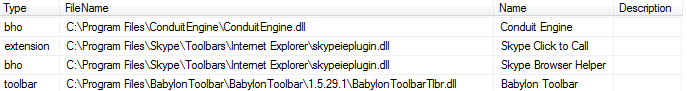
\includegraphics[scale=.8,angle=0]{figures/db_addons_snapshot.png}
\end{small}
\caption{An example SQL table}
\label{fig:db_addons_snapshot}
\end{figure}

The field values correspond to raw information extracted from the users' machines. Accordingly, it lacks normalization. Figure \ref{fig:addons_versioning_snapshot} \textcolor{red}{also here: use examples that include non-empty description values} illustrates the variability across records, which we consider to be co-referent as they describe the same addon. As shown, there are differences across individual records with resepct to the path in which the add-on is installed on the local machine, as well as the version number (e.g., 1.8.7.2 vs. 1.8.4.9 in the figure), name and description. Furthermore, the user base is international, and is accordingly multi-lingual.  \textcolor{red}{Say a bit more about the data: is there any add-on attribute that is always populated? path perhaps? how often is the add-on name or description left empty?}

\begin{figure}[t]
\centering
\begin{small}
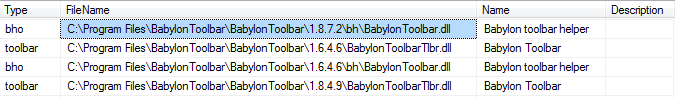
\includegraphics[scale=.8,angle=0]{figures/addons_versioning_snapshot.png}
\end{small}
\caption{An example SQL table with different versions for same addons}
\label{fig:addons_versioning_snapshot}
\end{figure}

Finally, we note another characteristic of interest of this data.  Since the add-ons lists per user are updated on a daily basis, it is straightforward to derive add-on changes (installation and removal) over time. However, there is no tracking of user actions or other programs actions. It is therefore impossible to determine which party initiated any of the status changes; for example, we cannot infer whether a particular addon has been removed (or installed) by the user or automatically, by hostile/protecting program. 

\section{Experimental data}

For the purposes of this study, we consider a subset of the data, including all of the records collected over a  period of two months between Aug. 1 2013--Oct, 1, 2013. Overall, this dataset contains 17,942,715 daily user--add-on associations. It consists of 907,844 users \textcolor{red}{are these users unique? probably not} and 456,458 addons \textcolor{red}{how come the number of addons is smaller than the number of users?}. Figure \ref{fig:user_addons_histogram} shows the distribution of the number of add-ons installed daily per user. As shown,  most users have between 9 and 21 addons installed on their PCs.

\begin{figure}[t]
\centering
\begin{small}
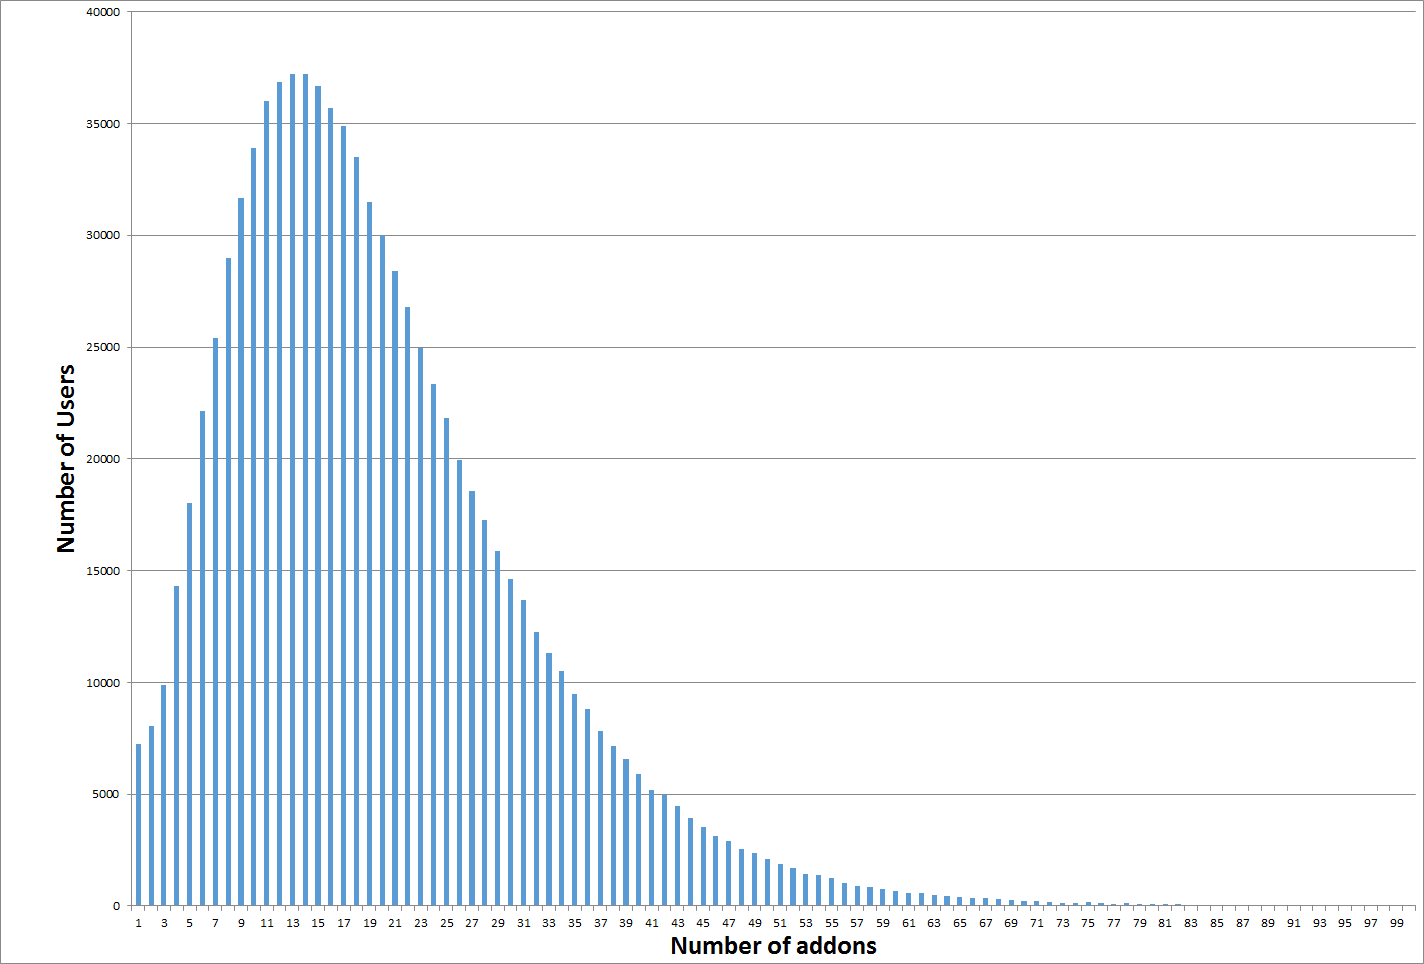
\includegraphics[scale=.9,angle=0]{figures/user_addons_histogram.png}
\end{small}
\caption{Number of addons per user distribution}
\label{fig:user_addons_histogram}
\end{figure}

In order to enable assessment of textual similarity for record co-reference purposes, we further processed the fields descrbing each add-on mention into a bag-of-words. This gives rise to another lexical object type, representing {\it terms}. For examples..

In converting text strings into individual {\it terms}, in addition to word tokenization, text cleanup and normalization steps were applied. Specifically, we removed some non-ASCII characters, originally added for encryption purposes on the server side prior to storing that data in SQL tables. Likewise,  Windows shortcuts for full paths have been removed (e.g., VIDEOD$\sim$1 and VIDEOD$\sim$2 and VIDEOD denote the same path), and so forth. Finally, all strings were converted all strings to lower case, since capitzliation is meaningless in this case. \textcolor{red}{How many unique terms did we get?}


\section{Graph representation}

\begin{table}[t]
\begin{center}
\begin{small}
\begin{tabular}{llll}
\hline 
\textbf{source type} & \textbf{edge type} & \textbf{target type} \\
\hline
{\it user} & has-add-on & {\it add-on} \\
\hline
{\it add-on} &  has-add-on$^{-1}$ & {\it user} \\
{\it add-on} & has-term & {\it term} \\
\hline
{\it term} & has-term$^{-1}$ & {\it add-on} \\
\hline
\end{tabular}
\end{small}
\end{center}
\caption{\label{tab:graph_structure} The graph node and directional edge types}
\end{table}

We compactly represent the dataset using a relational graph. Each node in the graph represent a unique, typed,  object.  Concretely, the graph includes the following node types:
\begin{itemize}
\renewcommand{\labelitemi}{$\bullet$} 
\item {\it User} - this node represents user by his unique user id. 
\item {\it Add-on} - this node represents unique addons, where an {\it add-on} is defined as the concatation of all its attributes, namely, file path, addon name and description.
\item {\it Terms} 
\end{itemize}
Directional edges link node pairs.
Table \ref{tab:graph_structure} details the types of edges, representing a variety inter-object relationships, which are derived directly from the relational database structure.
First, we represent the structural relationship between each user and the {\it add-ons} installed on his PC via the {\it has-add-on} edge type, originating at the {\it user} node. An inverse relation exists between each {\it add-on} node and the {\it users} that it is known to be installed at. 
In addition, as described above, each {\it add-on} is associated with its bag of terms representation. Concretely, each {\it add-on} node is linked to {\it terms} contained in either of its attributes over the {\it has-term} relation. Inversely, each {\it term} node is linked to {\it add-ons} that contain it over {\it has-term$^{-1}$} relation.



\iffalse
\begin{small}
\begin{enumerate}[(a)]
\item Go over all users, for each user create a graph node. Graph node name for a user has a prefix "u-" appended to user ID, for example u-00004c1b-8ffc-4ca4-b406-a27e436fa34a node.

\item For each user, go over all its add-ons.
\item For each addon create a graph node, graph node name has a suffix "a-" and appended all addon attributes. For example "a-c:/programfiles(x86)/skype/toolbars/internetexplorer/skypeieplugin.dll"
\item For each addon create term nodes according to its attributes, each term node has prefix "w-" and appedned with a term. For example the addon above would create 6 term nodes:
\end{enumerate}
\end{small}

\begin{itemize}
\renewcommand{\labelitemi}{$\bullet$} 
\item "w-c:"
\item "w-programfiles(x86)"
\item "w-skype"
\item "w-toolbars"
\item "w-internetexplorer"
\item "w-skypeieplugin.dll"
\end{itemize}
%\end{enumerate}
User has edges to all its addons and addon has edges to all it terms, all edges are bi-directional.\\
We have added additional steps for data cleanup.
\fi

\begin{figure}
    \centering 
    \begin{tikzpicture}[
      thick,
      acteur/.style={
        circle,
        fill=black,
        thick,
        inner sep=2pt,
        minimum size=0.2cm
      }
    ] 
      \node (a1) at (5,2.5) [acteur,label=u-00004c1b-8ffc-4ca4-b406-a27e436fa34a]{};
      \node (a2) at (2.5,2.5)[acteur,label=below:a-c:/programfiles(x86)/skype/toolbars/internetexplorer/skypeieplugin.dll]{}; 
      \node (a3) at (-5,0) [acteur,label=below:w-c:]{}; 
      \node (a4) at (-5,1) [acteur,label=w-toolbars]{}; 
      \node (a5) at (-5,2) [acteur,label=w-internetexplorer]{}; 
      \node (a6) at (-5,3) [acteur,label=w-skypeieplugin.dll]{}; 
      \node (a8) at (-5,4) [acteur,label=w-skype]{}; 
      \node (a9) at (-5,5) [acteur,label=w-programfiles(x86)]{}; 
      
      \draw[blue] (a1) -- (a2); 
      \draw[blue] (a2) -- (a3);
      \draw[blue] (a2) -- (a4);
      \draw[blue] (a2) -- (a5);
      \draw[blue] (a2) -- (a6);
      \draw[blue] (a2) -- (a9);
      \draw[blue] (a2) -- (a8);

    \end{tikzpicture} 
    \caption{An example graph view}
    \label{fig:sample_graph}
  \end{figure}
 
  \begin{figure}
    \centering 
    \begin{tikzpicture}[
      thick,
      acteur/.style={
        circle,
        fill=black,
        thick,
        inner sep=2pt,
        minimum size=0.2cm
      }
    ] 
      \node (u1) at (5,4) [acteur,label=u-1]{};
      \node (u2) at (5,0) [acteur,label=u-2]{};
      
      \node (a1) at (2.5,3)[acteur,label=below:a-1]{}; 
      \node (a2) at (2.5,4)[acteur,label=below:a-2]{}; 
      \node (a3) at (2.5,5)[acteur,label=below:a-3]{}; 
      \node (a4) at (2.5,2)[acteur,label=below:a-4]{}; 
 
      \node (w1) at (-3,1) [acteur,label=w-1]{}; 
      \node (w2) at (-3,2) [acteur,label=w-2]{}; 
      \node (w3) at (-3,3) [acteur,label=w-3]{}; 
      \node (w4) at (-3,4) [acteur,label=w-4]{}; 
      \node (w5) at (-3,5) [acteur,label=w-5]{}; 
      \node (w6) at (-3,0) [acteur,label=w-6]{}; 
      
      \draw[blue] (u1) -- (a1); 
      \draw[blue] (u1) -- (a2); 
      \draw[blue] (u1) -- (a3);
      \draw[blue] (u2) -- (a4);
      \draw[blue] (u2) -- (a2);
      
      \draw[blue] (a1) -- (w1);
      \draw[blue] (a1) -- (w2);
      \draw[blue] (a1) -- (w3);
      
      \draw[blue] (a2) -- (w1);
      \draw[blue] (a2) -- (w3);
      \draw[blue] (a2) -- (w4);
      
      \draw[blue] (a3) -- (w1);
      \draw[blue] (a3) -- (w2);
      \draw[blue] (a3) -- (w3);
      \draw[blue] (a3) -- (w4);
      \draw[blue] (a3) -- (w5);
      
      \draw[blue] (a4) -- (w6);
      \draw[blue] (a4) -- (w2);
      

    \end{tikzpicture} 
    \caption{An example graph view 2}
    \label{fig:sample_graph2}
  \end{figure}
  
Figure \ref{fig:sample_graph} \textcolor{red}{It would be good to include another add-on in the figure, or at least, a more interesting add-on, which also inlcudes a name and description} illustrates the graph generation process. Given a user, it is represented by a graph node, where we append the prefix "u-" to the user ID in order to simplfy the identification of node types; for example, in the figure, the user is denoted by the node `u-00004c1b-8ffc-4ca4-b406-a27e436fa34a'. For each user, we iterate over all its add-ons, where each unique add-on is mapped to a graph node. {\it Add-on} graph node names include the prefix "a-", followed by a concatenation of the addon attribute values; in the figure, a single add-on exists, for which only path infomration is availabe, where the respective node name is `a-c:/programfiles(x86)/skype/toolbars/internetexplorer/skypeieplugin.dll'. Finally, each {\it add-on} node is mapped to {\it term} nodes. The term nodes start with the prefix "w-". \textcolor{red}{Did you apply stemming?}; for example, the {\it add-on} node in the figure is linked to six term nodes, wich resulted from the string tokenization and processing. 
  
The graph representation of this data has several advantages. Besides being compact, we expect similar entities to reside in high proximity to each other in the graph. For example, the {\it add-ons} named `Skype-US' and `Skype-UK' have non-identical names; however, they share the term `skype', indicating in this case that they are variants of the same add-on. Figure \ref{fig:terms_layer} illustrates how the representation of the full strings results in isolated graph segments, whereas adding the terms nodes yields a connected graph, where the two add-ons are linked over a path that traverses the "Skype" term node.

\begin{figure}[h]
\centering
\begin{subfigure}[b]{0.49\textwidth}
	\centering
	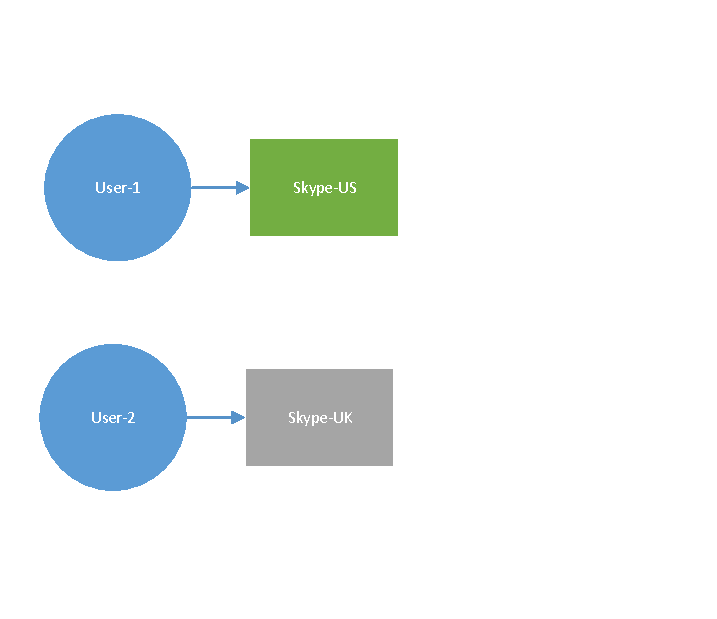
\includegraphics[width=\textwidth]{figures/skype_exampe1.pdf}
	\caption{Without terms layer}
%	\label{fig:skype-no-terms}
\end{subfigure}
\begin{subfigure}[b]{0.49\textwidth}
	\centering
	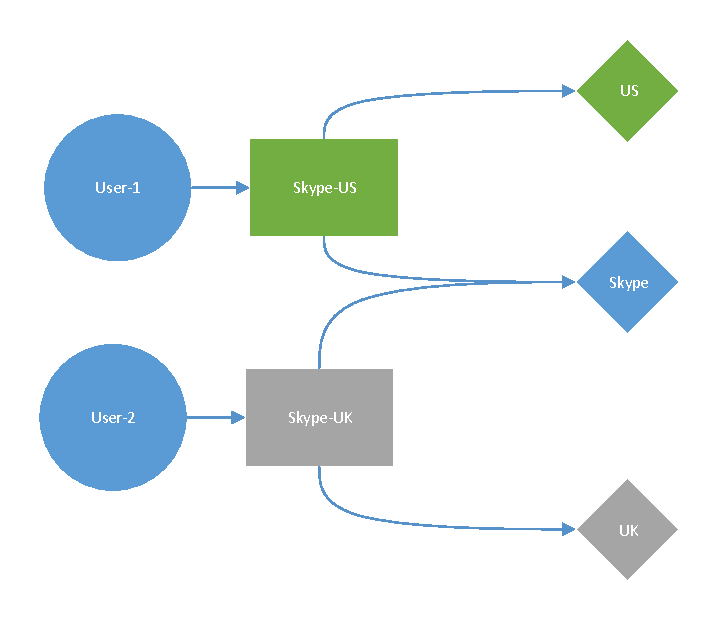
\includegraphics[width=\textwidth]{figures/skype_exampe2.pdf}
	\caption{With terms layer}
%	\label{fig:skype-with-terms}
\end{subfigure}
	\caption{Terms layer example}
	\label{fig:terms_layer}
\end{figure}
  
Figure \ref{fig:sample_graph2} shows another toy graph, demostrating another aspect of inter-user similarity reflected as connectivity patterns in the graph. This gtaph includes two users named shortly as `u-1' and `u-2'. The two users are similar in that they share two add-ons, `a-1' and `a-2'. In addition, while {\it add-ons} `a-3' and `a-4' are distinct from each other, these add-on nodes are connected via the common term node `w-2'. 

We will apply random walks in the graph in order to assess similarity, or relatedness, between users and add-ons.  

\chapter{General Approach}
\label{sec:method}
In this chapter we will present the algorithms we implemented for this thesis.
\section{Baseline algorithms}
We chose to use two algorithms to test our algorithms, a popularity baseline and an pagerank ranking based baseline. The popularity baseline is a simple recommendation technique and the reason that we chose this method was its speed and simplicity. This allowed us to iterate quickly in the early stages of our research. The item similarity baseline is a more complicated algorithm and was used as a more realistic test of the performance the algorithms. Because the largest datasets we worked with contained hundred of thousands of users and tens of millions of items, we had to make sure that the
baseline algorithms were implemented in a high performance, parallel or distributed
environment. We chose to use igraph \citep{igraph}, a high-performance, parallel machine learning framework. This allowed us to focus our efforts on the development of our algorithms and not the baseline algorithms.
\subsection{Popularity}
The popularity algorithm is one of the simplest one can employ for recommending items, as it simply recommends the most popular items in the dataset to all the users. The popularity of the items is determined by the total number of user for each addon in the dataset, and all the users are presented with the same recommendation list, where the items are ranked according to their popularity. Despite its
simplicity, the popularity algorithm can perform reasonably well.
Another advantage for this algorithm is lack of parameters and the fact that due to its simplicity we are able to make recommendations for datasets containing hundreds of thousands of users and tens of millions of items very fast. Both of these factors contributed in making experimentation much easier, an important factor for a baseline algorithm.
This benefit however comes at a cost for the quality of the recommendations. Since the algorithm performs no personalization in the recommendations made, all users are presented with the same recommendation list.
\subsection{Prediction based on PageRank scores}
For each addon we have calculated its PageRank score by running the regular PageRank algorithm over the whole user addon graph. Now, like in \autoref{sec:PPR_addons_method}, when we are predicting the missing add-on, we are looking at the addons ranking list (the ranking is according to PageRank scores) and check the Recall@K. This measure seems to give similar results as the Popularity baseline.

\section{Personalized PageRank addons analysis}
\label{sec:PPR_addons_method}
The PageRank that is described in \citep{page1999pagerank} gives a universal score for the nodes in a graph. It is however possible to change the calculations so that the results will reflect someone’s personal preferences. In the PageRank formula the teleportation vector $\vv{u}$ has a great influence on determining the outcome. The biasing of the PageRank by this vector is first suggested in \citep{brin1998can}, and thereafter explored many times (\citep{haveliwala2002topic},\citep{haveliwala2003topic},\citep{haveliwala2003analytical}).In this thesis the goal of biasing the PageRank with the teleportation vector is to personalize the user addons of choice results. PageRank exists for any graph and not just the web graph. PageRank on a graph produces an importance score for each node, and this places PageRank amongst a class of network analysis techniques \citep{brandes2005network} known as centrality measures or indices \citep{koschutzki2005centrality}.
Instead of looking at a “randomsurfer” on the web, the non-web PageRank models a random walk on the graph. The behavior of the walk is the same as the random surfer: with probability $\alpha$ the walk continues along an edge
of the graph and with probability 1-$\alpha$ the walk jumps to a random node in the graph. Personalized PageRank is an important extension of PageRank model, in which the surfer does not randomly restart browsing anywhere on the web after choosing not to follow a link. Rather, the surfer in this new model restarts at one of only a few pages. If the pages relate to one person, then the resulting PageRank vector is called a personalized PageRank vector. If the pages are topically related, then the vector may be called a topic-specific PageRank vector.
In \citep{freschi2007protein}, the authors used the Personalized PageRank model, which they call ProteinRank, to predict protein functions. The Personalized PageRank model seems to perfectly apply to our set of problems as well. We are dealing with users and looking for their personal preferences in browsers extensions, we are also interested in Company based addons propagation in users network. All our dataset was transformed to undirected graph, where user nodes are connected to addon nodes according to their relationship in the original dataset, e.g. each user node has an edge connected to addon node if this user has this addon installed in its ecosystem. Since our goal is to determine/predict a missing addon in user ecosystem, the seed nodes for the personalization vector would be the specific user addons, our hypothesis is that a higher the PageRank score suggests a higher relevance of an addon to the specific user. We would run multiple experiments to show the correctness of our hypothesis.

\iffalse
\subsection{Support Vector machine}
First we have tried running analysis on our data using SVM. We were trying to classify users that are staying long in user ecosystem and those that churn immediately, lately this would turn to Clash prediction.\\
We have defined training data as follows - positive examples are the users that have stayed at the system more than three days and others are negative example. We have used a popular libSVM tool to run the analysis.\\
The training very long time and gave no results, trying to run SVM with another kernel did not help either - and every run took a few days to finish. Then we've decided to find another way to represent our data.
\subsection{GraphChi}
\subsection{iGraph}
\fi

\section{Similarity in graphs using Personalized PageRank}
\iffalse
\textcolor{green}{\textit{Einat: 
This may be a good place to introduce PPR. This algorithm will be used
in both recommendation and clash prediction experiments.}}\\
\fi
Personalized PageRank
is an extension of the famous PageRank algorithm \cite{page1999pagerank}, both of
which are based on a random surfer model. To understand Personalized PageRank, we first review the original
PageRank briefly. A random surfer starts at any node on the
graph. At each step, with a probability of 1−$\alpha$ the surfer moves to
a neighboring node randomly, and with a probability of $\alpha$ he teleports to a random node on the graph. This process
is repeated until the walk converges to a steady-state. The stationary
probability of the surfer at each node is taken as the score of
the node. However, this form of score is purely based on the static
link structure, indicating the overall popularity of each node on the
graph, without tailoring to a specific query node.\\
In contrast, Personalized PageRank enables query-sensitive ranking,
in the sense that we can specify a query node to obtain a “personalized”
ranking accordingly. It is based on the same random
surfer model of the original PageRank, except when the surfer teleports,
he always prefers the query node \textit{q}. Specifically, at each
step, with probability $\alpha$ the surfer teleports to \textit{q} instead of a random
node, thus visiting the neighborhood of \textit{q} more frequently.
Thus, the stationary distribution, called a Personalized PageRank
Vector (PPV), is biased towards \textit{q} and its neighborhood, which can
be interpreted as a popularity or relevance metric specific to \textit{q}.
More generally, a query \textit{q} can comprise multiple nodes on the
graph, such that in the teleportation the surfer can jump to any
node in \textit{q}. Fortunately, the computation for a multi-node query is
no more difficult than for a single-node query due to the \textit{Linearity Theorem} \citep{jeh2003scaling}, as the PPV a multi-node query is a simple
linear combination of the individual PPV each node in the
query.
\iffalse
A personalized
PageRank vector, also known as
a random-walk with restart (RWR), is the stationary distribution of a random
walk that, with probability $\alpha$ follows a step of a random walk and with probability (1−$\alpha$) jumps back to a seed node.
If there are multiple seed nodes, then the choice is usually
uniformly random. The set of these seeds is called personalized PageRank Vector (PPV).
\fi

\chapter{The missing addon in User ecosystem}
\label{chap:user_ecosystem}
\iffalse
\textcolor{green}{\textit{Einat: Start by introducing the problem, why it is interesting..}}\\
\fi
In this chapter we present the experiment results and analyze the performance of the algorithms.
Consider a user-addons network
with users and addons as nodes, where users are connected to its addons and are connected between them via add-ons. Given a user
in the network, how can we detect some potential addons that would be relevant for him? Taking the user addon nodes as user ecosystem and detecting which node is missing in this ecosystem would answer this question. We are using a Personalized PageRank over the a graph of users and addons (seen as global ecosystem) and taking a specific set of user addons as PPR input query, a ranking over all the
other addon nodes can be leveraged for the detection of missing addon in user ecosystem.\\
In the above scenario, the rankings are specific to the dynamic
queries, reflecting the “relevance” of nodes to the query node. As a
well-studied graph ranking algorithm, Personalized PageRank \citep{page1999pagerank} is effective in calculating such query-specific relevance based
on the link structure of the graph. In this paper, we use the rankings of Personalized PageRank, as a criteria for recommending an addon.

\section{Experimental setup}
\iffalse
\textcolor{green}{\textit{Einat:Explain how the dataset was constructed - we removed one addon per
user; use the remaining addon as a query.. how many queries?}}\\
\fi
ADD THIS SOMEWHERE: On the other hand, many addons have a file-system path in their name, such as C://Program Files (x86)//..., thus we have hypothesized that connecting these addons into term nodes will create massively connected addons while they don't actually have something in common (besides being installed on user PC). We have tested this issue in two ways. First, we have ran experiment comparing results on graph with removed addons prefix that contain a common prefixes like C://Program Files (x86) and on graph where addons remained with full paths. Second, we have ran experiment on a graph when we have removed high degree nodes (higher than 500) and on graph with all nodes, and compared the results. Removing high degree node should only result in only a small approximation error[cite Purnamrita Sarkar], while improving the performance and giving equal opportunity for low-degree nodes.
Another issue we had to overcome was the same addons, but with different versions. Addons with different version usually resulted in slightly different addon name, this difference could be at the name itself or in path leading to this addon. Splitting the addon nodes into terms should elegantly overcome this obstacle, since the addons will differ only slightly because of its versions.Thus users having the same addon but with different versions will still be strongly connected.


Given the large scale of our graph - 1,331,814 nodes and 18,552,622 edges , and our need to execute the algorithm multiple number of times (thousands), we needed to find a fast and memory wise implementation of Personalized PageRank.

We have chosen igraph \citep{igraph} which is a library for creating and manipulating graphs.iGraph uses internally ARPACK package which is a numerical software library written in FORTRAN 77 for solving large scale eigenvalue problems (used also in Mining and Analyzing Social Networks book). ARPACK uses an implicitly restarted Arnoldi method to calculate PageRank. igraph expects as an adjacency list of numeric vertices. We have created a unique number for each node and store the mapping to an actual node name in a separate file. Since the whole graph is loaded into memory, we had to be very careful with memory management (every very small leak would cause a serious global memory leak). We also had to compile a 64bit version of igraph - since 32 bit version failed running - it could not acquire enough memory.

The dataset is constructed as following:\\
\iffalse
\textcolor{green}{\textit{Sela: Add visible graphics to show the nodes and its connections:}}
\fi
\begin{enumerate}[(a)]
\item Pick uniformly at random a user node at the graph, find all its addon nodes.
\item Pick uniformly at random an addon node from the list of nodes found above.
\item Remove this node - since the only connection between a user node and the addon node is the edge between them, by simply deleting this edge we are removing this addon from user profile.
\item Now, the remained addons are the seeds of PPR vector.
\end{enumerate}

The output of our algorithm is a ranked list of all add-ons. The addons are ranked according to their PageRank score.

\iffalse
\textcolor{green}{\textit{Einat:Used Personalized PageRank -- which parameters? how were the paramater
values set?}}
\fi

After PPR ran we have every addon (actually every node in graph) has a pagerank score. Obviously the addons that were at the personalized - the user addons - are likely to be ranked very high. But we have removed one addon from the user set of addons, now its addon has no connection to user addons except for connections that pass by other users or terms nodes. So after we have removed this addon node from the user, it is no different than other 200 thousands addon nodes. Now, we want to see what is the rank of this addon that we have removed, the higher it would be the better our recommendation algorithm works. Since, lets say it is ranked in 8th position, not taking into account the ranking position of the original user addons, then we could recommend to user top ten scored addons and with high probability user will find a usefull addon between this ten.\\
\iffalse
\textcolor{green}{\textit{Sela: Example:}}
\textcolor{green}{\textit{Einat:How was evaluation conducted? cross validation.. using MAP meausre(?)
(can include a description of MAP as an appendix)}}
\fi
\section{Ranking measures}
\label{sec:ranking}
\paragraph{Recall at k - R@k}
Recall-at-k (Recall@k) is the fraction of the documents relevant to the query that are successfully retrieved out of the first k returned. Recall@k is therefore a highly localized evaluation criterion, and captures the quality of rankings for applications where only the first
few results matter.For recommendation systems, users usually will only view several top ranked candidates. Therefore whether
the correct addon exists in the top ranked candidates is important, and Recall@k is designed for measuring this.

\begin{displaymath}
 Recall = \frac{number \, of \, relevant \, documents \, retrieved}{number \, of \, relevant \, documents}
\end{displaymath}
\iffalse
\begin{displaymath}
 Precision = \frac{number \, of \, relevant \, documents \, retrieved}{number \, of \, retrieved \, documents}
\end{displaymath}
\fi
\paragraph{Mean Reciprocal Rank}
Recall@k considers whether correct addon is in the top
k results, but it does not consider the exact ranking position
of the correct addon. Mean reciprocal rank (MRR) \citep{voorhees1999trec} is a well-known evaluation metric in Information
Retrieval (IR) and is typically used to evaluate the position of the first correct candidate. Given the analogy between query-document
search and user-item recommendation, we can define the Reciprocal Rank (RR) for a given recommendation
list of a user, by measuring how early in the list (i.e. how highly ranked) is the first relevant recommended item. The MRR is the average of the RR across all the recommendation lists for individual users. MRR is a particularly important measure of recommendation quality for domains that usually provide users with only few but valuable recommendations
(i.e., the less-is-more effect \citep{chen2006less}), such as friends recommendation in social networks where top-X performance is important.
\begin{displaymath}
 MRR = \frac{1}{Q} \times \displaystyle\sum\limits_{q=1}^{Q} \frac{1}{rank(1^{st} \, relevant \, result \, of \, query \, q)}
\end{displaymath}

\paragraph{Evaluation Metrics}
For evaluating our model we use the standard information retrieval measures. For every user
we compute: (1) recall at rank k (P@k) for our task is
defined as the fraction of rankings in which the correct addon is ranked in the top-k positions, (2) Our recommendation is correct when the correct addon is present in
the ranked set of add-ons. The mean reciprocal rank (MRR)
is the inverse of the position of the first correct addon in the
ranked set of addons produced by our model\\
For each user, we have chosen, uniformly at random, one of its addons and completely removed this addon connections to this user. Now, we have added all user addons to PPR vector and executed PPR.
We ran the experiments with teleport probability $\alpha$ = 0.85.
While we were looking for best setup for addons recommendation system, we have also observed our algorithm behavior in different kind of setups.
\iffalse
\textcolor{green}{\textit{Sela: Another possible graph is distribution of users that we have correctly found the missing addon and user number of addons, from what I recall, the fewer addon user is having - the higher the chances to find a good addon}}\\
\fi
\paragraph{Why terms nodes doesn't really matter}
Every addon has in its neighborhood many nodes which it is connected to. Many of them are USER nodes and only very few are TERM nodes. For example, 203 neighbors with 200 are user nodes and 3 are term nodes. Given that we are running Personalized pagerank and supposedly many users are the same for the vector of current addons, than most of the weight will go via the users and terms will get very small weight to traverse. While term node might be connected to many many other addons - it almost doesn't get any weight from them since we are running Personalized PageRank and not regular PageRank most of the weight is concentrated in the personalized vector - which contains only current user addons and not terms.
\paragraph{Compared methods}
In every experiment we are comparing the baseline methods to our method.For each of the methods we report Recall@10, Recall@50, Recall@100 and MRR as described at \autoref{sec:ranking}
\paragraph{Experiments parameters}
In every experiment we have a few parameters that we can change in order to tune and compare our method performance:
\begin{itemize}
\renewcommand{\labelitemiii}{$\diamond$}
\item Graph with addons that include full path or only the addon file name - as described in \autoref{sec:datasets}, we have decided to test our method when using only addon filename as node in the graph and when using full addon path as node in the graph.
\item Removing high degree nodes from the graph or not. We hypothesize that in addons/users ecosystem high degree nodes insert more noise in random walk than they contribute to correct pagerank execution. We have observed that high degree nodes are usually common nodes that will contribute more to locality instead of letting pagerank flow reach the hypothesized nodes. While removing high degree node might obviously hurt the popularity baseline performance.
\item Minimal number of addons user must have for running our prediction method. Clearly, the absolute minimum is two since when 
\end{itemize}

\section{Analysis}


\iffalse
\paragraph{Graph of addons without paths and without popular nodes}
\fi
In this thesis a great number of experiments were conducted, each validating a specific aspect of use ecosystem and trying to maximize our prediction accuracy and correctness. We have begun by removing all nodes from the graph that have a degree higher than 500. We hypothesize that in addons/users ecosystem high degree nodes insert more noise in random walk than they contribute to correct pagerank execution. We have observed that high degree nodes are usually common nodes that will contribute more to locality instead of letting pagerank flow reach the hypothesized nodes. In general, a high degree node could mean one of two things:
\begin{itemize}
\renewcommand{\labelitemiii}{$\diamond$}
\item If the high degree node is a term node, it means that this term is very popular between addon nodes and most probably it won't contribute for prediction of user addon.
\item If the high degree node is an addon node, it means that this addon is very popular among the users and, as with term nodes, it could destruct the weight flow and also it could just recommend an already very popular item to a user.[SELA Improve]
\end{itemize}
Moreover, it is important to remember that we are experiencing with the Personalized PageRank and our hypothesis is that if the teleportaion vector in some way simulates user ecosystem, the PageRank flow would grant a missing node a high rank, mainly because of the seed nodes which belong to the same user. Thus, due to PageRank weight propagation technique, high degree node would actually reduce the influence of the original seeds.

We have also chosen the users that have at least two addons installed on their computer. This restriction is very fundamental since we have no way (at least at our algorithm) to recommend an additional addon to user having only one addon, our way of knowing that we have predicted a correct addon is by removing one addon from all user addons and running PPR from the remaining add-ons. As with all our experiments, unless stated otherwise, we have picked uniformly at random one thousand users and conducted the experiment. As shown at \autoref{fig:minlen2remove500Recall}, our algorithm has correctly predicted a missing addon at top-10 ranking list addons, in {$\sim$}42\% cases. It is also greatly outperforms the baseline benchmark. We have also compared the Mean Reciprocal Rank (MRR) of our algorithm and the baseline as shown in \autoref{fig:minlen2remove500MRR}.

\begin{figure}[h]
\centering
\begin{subfigure}[b]{0.49\textwidth}
	\centering
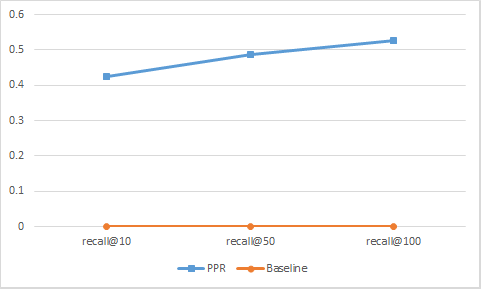
\includegraphics[scale=0.49]{figures/minlen2remove500.png}
\caption{Recall@K}
\label{fig:minlen2remove500Recall}
\end{subfigure}
\begin{subfigure}[b]{0.49\textwidth}
	\centering
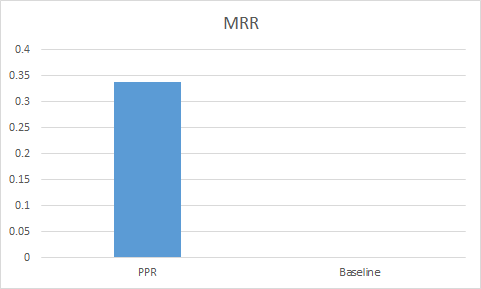
\includegraphics[scale=0.49]{figures/minlen2remove500MRR.png}
\caption{MRR}
\label{fig:minlen2remove500MRR}
\end{subfigure}
	\caption{Graph without paths without popular nodes}
	\label{fig:minlen2remove500}
\end{figure}

\begin{figure}[h]
\centering
\begin{subfigure}[b]{0.49\textwidth}
	\centering
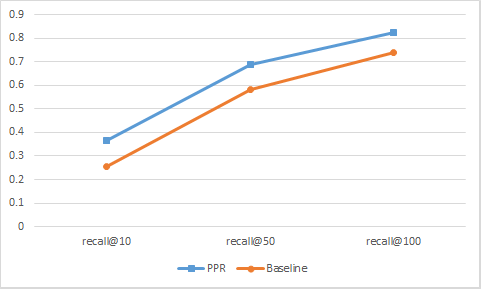
\includegraphics[scale=0.49]{figures/minlen2noremove.png}
\caption{Recall@K}
\label{fig:minlen2noremoveRecall}
\end{subfigure}
\begin{subfigure}[b]{0.49\textwidth}
	\centering
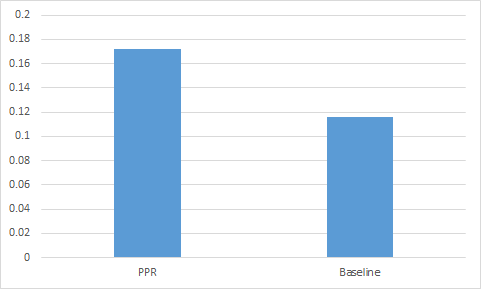
\includegraphics[scale=0.49]{figures/minlen2noremoveMRR.png}
\caption{MRR}
\label{fig:minlen2noremoveMRR}
\end{subfigure}
\caption{Graph without paths with popular nodes}
	\label{fig:minlen2noremove}
\end{figure}

Now, we've wanted to check how the high degree nodes would influence the prediction algorithm, so we've conducted the same experiment as in \autoref{fig:minlen2remove500Recall} but without removing any node from the original graph, the results are shown at \autoref{fig:minlen2noremove}. As we observe at \autoref{fig:minlen2noremoveRecall}, the Recall@10 prediction has dropped from {$\sim$}44\% to {$\sim$}36\%, while Recall@50 and Recall@100 have improved. One possible explanation of this behavior is that Recall@10 is less subtle to popular addons than the Recall@50 and Recall@100, thus while popular nodes can frequently enter the positions in top-50 or top-100 ranking lists, its harder to enter the top-10 rankings where the actual real prediction lies.[SELA Improve]
\paragraph{High degree nodes}
High degree nodes in our graph typically represent a very popular addons or a term. We were considering how to treat this kind of nodes, on the one hand these nodes are part of the graph and should be treated like all other nodes. On the other hand, given the addon popularity, it is unfair to predict it - it is somewhat trivial. We've conducted all of the experiments in both ways - with and without high degree nodes.But it is our opinion that the high degree nodes should be treated in a similar way to how the stop words in lexical analysis are treated. Since the stop words has no interest for the prediction algorithms it is usually removed. We've observed, see \autoref{fig:nodes_degree_dest}, that the nodes degree distribution follows Zipf's law distribution.
\begin{figure}[h]
\centering
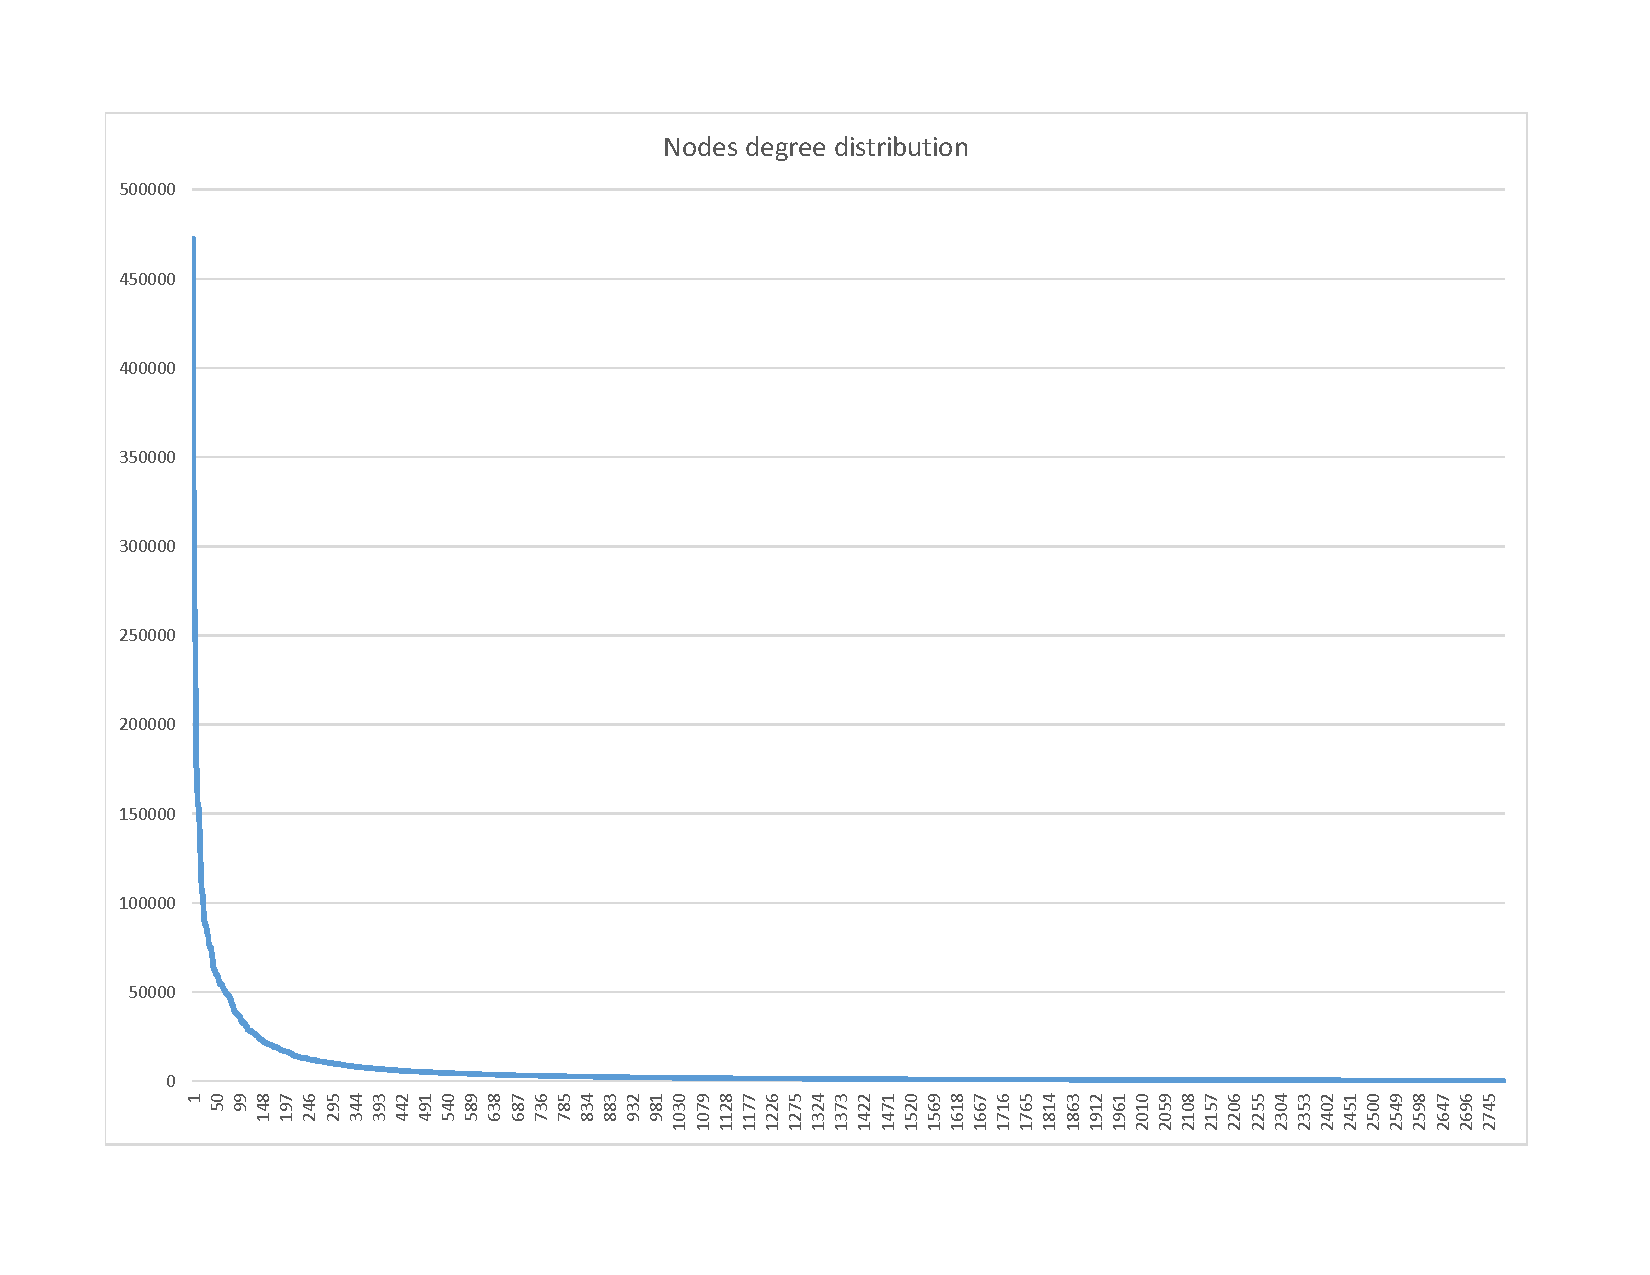
\includegraphics[width=\linewidth]{figures/nodesDegreeDest.pdf}
\caption{Nodes degree distribution}
\label{fig:nodes_degree_dest}
\end{figure}
\par
Given the differences between the algorithms scores, it is a good place to mention the SD and the SEM of the experiments, see \autoref{table:std_ste}.
\begin{table}[h]
\centering
\caption{Standard deviation and Standard error of the Mean}
\label{table:std_ste}
\begin{tabular}{|c|c|c|c|} \hline
 & Recall@10 & Recall@50 & Recall@100\\ \hline
SD & 0.001773 & 0.002601 & 0.005279\\ \hline
SEM & 0.001024 & 0.001502 & 30.003048\\ \hline
MEAN & 0.358904 & 0.661086 & 0.80593\\ \hline
\end{tabular}
\end{table}

As mentioned at \autoref{sec:method}, the addons data as collected from the users refers to addons usually by full file system path, e.g. C:/Program Files/Skype/skype1.dll, While breaking this addon to term nodes this would create four nodes $C$,$Program Files$, $Skype$ and $skype1$. In \autoref{fig:minlen2noremove} and \autoref{fig:minlen2remove500}, we have chosen to remove the file system path from addon, hence the NoPath abbreviation, so we actually would have only one node $skype1$. We have also conducted \autoref{fig:minlen2noremove} experiment while not removing file system path from addon. The results are shown at \autoref{fig:minlen2noremoveWithPaths}.

\begin{figure}[h]
\centering
\begin{subfigure}[b]{0.49\textwidth}
	\centering
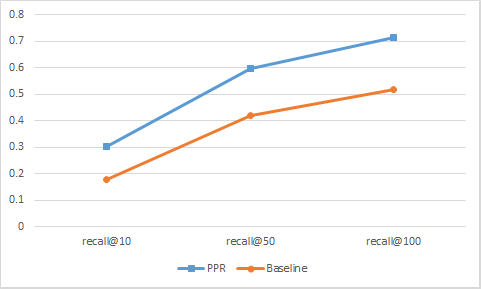
\includegraphics[scale=0.49]{figures/minlen2noremoveWithPaths.png}
\caption{Recall@K}
\label{fig:minlen2noremoveRecall}
\end{subfigure}
\begin{subfigure}[b]{0.49\textwidth}
	\centering
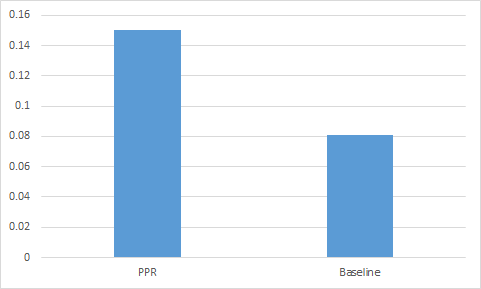
\includegraphics[scale=0.49]{figures/minlen2noremoveWithPathsMRR.png}
\caption{MRR}
\label{fig:minlen2noremoveMRR}
\end{subfigure}
\caption{Graph with paths with popular nodes}
	\label{fig:minlen2noremoveWithPaths}
\end{figure}

If we compare the results of the same run, as shown in \autoref{fig:with_without_paths_noremove}, we observe that adding addons paths hurts the performance, this can support our claim that high degree nodes, which obviously added when adding addons paths, disturb the PPR weight propagation from the real missing addons nodes. Interestingly, adding addons paths but removing high degree nodes improves the performance of our algorithm, see \autoref{fig:with_without_paths_remove500}. These two experiments, shown in \autoref{fig:with_without_paths}, support our claim that high degree nodes should be removed to improve prediction quality. Since, once they are removed, addition information about the user, like it paths, contributes to understanding and predicting its ecosystem state.

\begin{figure}[h]
\centering
\begin{subfigure}[b]{0.49\textwidth}
	\centering
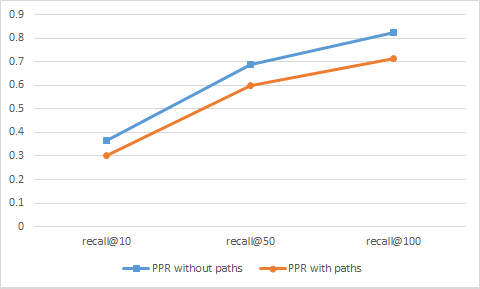
\includegraphics[scale=0.49]{figures/minlen2noremoveCompPaths.png}
\caption{With/without addon paths with popular nodes}
\label{fig:with_without_paths_noremove}
\end{subfigure}
\begin{subfigure}[b]{0.49\textwidth}
	\centering
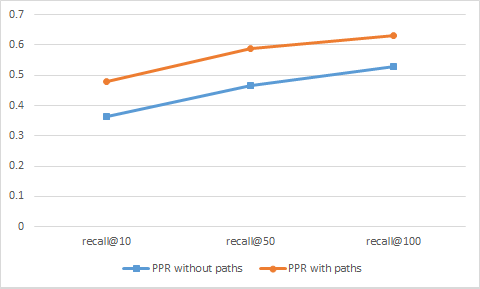
\includegraphics[scale=0.49]{figures/minlen5remove500CompPaths.png}
\caption{With/without addon paths without popular nodes}
\label{fig:with_without_paths_remove500}
\end{subfigure}
\caption{Comparing graph with/without addon paths}
	\label{fig:with_without_paths}
\end{figure}


As we have mentioned earlier, in order for our prediction algorithm to run, we require that user has at least two add-ons. At \autoref{fig:addonsNumberGraph},we are showing the affect number of addons that user have pre-installed on the algorithm accuracy. The \autoref{fig:addonsNumberGraph} graph shows that, while the prediction algorithm still performs on any number of pre-installed, its accuracy decreases as the number addons that user has, growth. One possible explanation to this behavior could be - if user addon is predicted, i.e. receives its PageRank score, mainly from other users that have a similar ecosystem - that the lesser addons user has the more unique its ecosystem.

\begin{figure}[p]
\centering
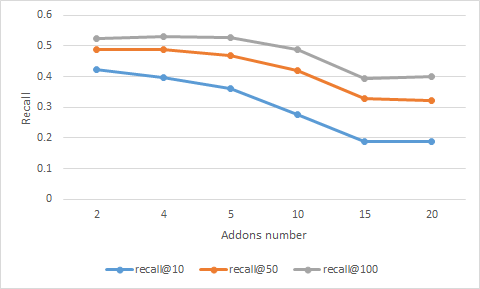
\includegraphics[scale=1,angle=0]{figures/addonsNumberGraph.png}
\caption{Effect of addon number on prediction accuracy}
\label{fig:addonsNumberGraph}
\end{figure}


As described in \autoref{sec:method}, we have added an additional layer of nodes to the graph - the term nodes. Now, we want check its efficiency on the prediction algorithm performance. As shown in \autoref{fig:with_without_terms}, adding term nodes has improved the prediction.

\begin{figure}[p]
\centering
\begin{subfigure}[b]{0.49\textwidth}
	\centering
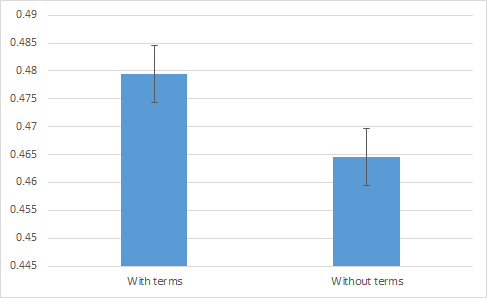
\includegraphics[scale=0.49]{figures/5addonswithoutTermsComp.png}
\caption{With/without term nodes with paths without popular nodes}
\label{fig:with_without_terms5}
\end{subfigure}
\begin{subfigure}[b]{0.49\textwidth}
	\centering
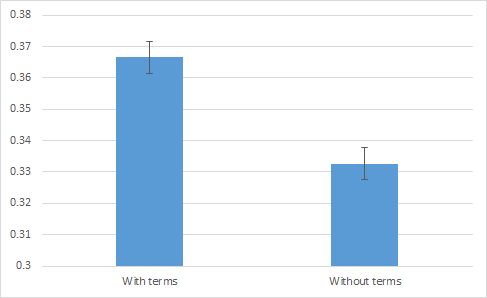
\includegraphics[scale=0.49]{figures/2addonswithoutTermsComp.png}
\caption{With/without term nodes without paths with popular nodes}
\label{fig:with_without_terms2}
\end{subfigure}
\caption{Comparing graph with/without addon paths}
	\label{fig:with_without_terms}
\end{figure}

We have also verified that user nodes are crucial for the prediction algorithm, as shown in \autoref{fig:nouserNoremove}.

\begin{figure}[h]
\centering
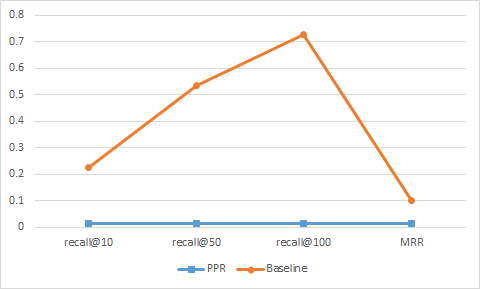
\includegraphics[scale=.8,angle=0]{figures/nouserNoremove.png}
\caption{Effect of user nodes on prediction accuracy}
\label{fig:nouserNoremove}
\end{figure}


\section{Discussion}
Our prediction algorithm performs best on full graph when highly connected nodes are removed, removing very highly connected nodes improves PPR convergence and reduces the noise in random walk.
Moreover, users that are having only two addons eases the prediction, which intuitively makes sense since the PPR personalization vector contains only one node. In experiment shown in \autoref{fig:addonsNumberGraph}, you can observe that picking users with higher number of pre-installed addons reduces the algorithm performance but still performs well. In experiment shown in \autoref{fig:with_without_terms}, you can observe the importance of term nodes, they improve connectivity between similar addons and thus improves our prediction rate. An obvious observation can be made from experiment shown in \autoref{fig:nouserNoremove}., graph without user nodes are almost not possible for recommender to find a missing addon node.




\chapter{PPR-based analysis of addon coexistence}
\label{chap:Symbiosis}

In this chapter, we investigate the addon coexistence phenomenon. We observe that some addons tend to coexist well with other addons, i.e. when addons of one company are installed on a user's PC, addons of another company have greater chances to be installed on the same machine.  This phenomenon often occurs when addons of some companies are distributed via third parties: addon installation is proposed to a user as a part of some other product installation process, for example, while the user installs Skype, the installation process suggests also installing Skype's `Click to Call' addon in all browsers. Another example is Google Toolbar: when the data for this paper was collected, Google distributed its toolbar in conjunction to installation of other products, such as Firefox or Winrar.

The opposite effect to coexistence can be observed as well: addons of one company have lower chances to exist on a machine if addons of another company are installed on this machine. For example, \emph{Avira AntiVirus}, which develops addons for all browsers, treats \emph{iMesh} addons as threats and removes them from the computer.

Companies that distribute browser addons are engaged in partnerships or compete with each other, such that the Web browser becomes a complex ecosystem similar in its characteristics to the biological environment of the nature. To illustrate this analogy, let us say that addon distributors correspond to biological species. An instance of an addon distributed by company $A$ can be viewed as a subject of species $A$ that coexists in the browser ecosystem with other subjects of the same or different species. Naturally, those subjects can live in symbiosis or in conflict with each other. We observe situations when addons of some companies get installed on a machine together with addons of other companies, which is analogous to a natural migration process when subjects of different species travel together. We also observe clash situations when an addon gets installed on a machine and ``kicks out'' addons of other companies, similarly to a competition phenomenon between different species in the nature. The user (the computer owner) is also playing an important role in the addon ecosystem: some users ``hunt down'' and remove addons that occasionally appear in the computer's browser; other users are more tolerant -- they let addons live in the browser for a long time and do not mind more addons to be added over time.

Needless to say, the life cycle of the addon ecosystem is mostly obscure for an outside observer. While some symbiosis effects are fairly visible to the users (e.g., in product installation processes), many others are hidden (e.g., undisclosed agreements between addon distributors) or implicit (two addons are statistically prone to coexistence). Clash effects, on the other hand, are almost always invisible. Besides a few well known conflicts between competing addon distributors that were widely covered in mass media \footnote{\url{http://finance.yahoo.com/news/babylon-shares-jump-yahoo-sticks-125203474.html}} [RON:citation needed], the competition is kept away from the eyes of general public. In this chapter, we disclose some of these effects and shed light on the entire addon ecosystem. 

The ability to detect and analyze a clash or symbiosis between addon distributing companies could turn handy for addon owners. 
A typical company that builds its business around developing and distributing addons (via a webstore, for instance), can benefit from information about a clash between their and someone else's addons, in four different ways.
First, such a clash may imply that the user prefers someone else's addon over their addon, so there might be a way to compare the two addons and  learn how to improve their value proposition. 
%Most probably, the user prefers the competitor's addon for a specific reason. In the Web browser ecosystem, identifying one's competitor is not an easy problem --- the clash information can help to solve this problem.
Second, the clash could mean that a newly installed addon is hostile to other addons in an illegal way, i.e. this is the addon --- and not the user ---- that uninstalls or sabotages another addon. Then, the distributor of the removed addon could report an abuse to the webstore owner.

Third, an addon developing company can ask a third-party distributing company not to install their addon on a machine that keeps the hostile addon. Since in most cases addon developers are paying distributors per install, this could decrease the developers' costs and improve their profits in a long run.
Fourth, a clash can occur between addons of seemingly non-competing companies. This can happen when something goes wrong in the distribution process and the problem slips off the company's radar. The addon ecosystem is complex enough to make the distribution monitoring barely possible. If an unintended clash gets detected, the owner of the affected addon can contact the owner of the hostile addon and ask to act.

[RON: We need to finish the story here. An intermediate conclusion and outline of the rest of the chapter?]
To the best of our knowledge, ours is the first study to research the addons ecosystem and its relations. Both the addons developers and security companies can benefit from this study and its conclusions.In the following sections,we will first describe the experimental setup for this chapter,in particular, the reasons behind its structure. We will then mention preliminary experimental efforts we have conducted before coming up with current experimental design. Following is the experimental design. In two sections that follows we describe our findings about symbiotic relationships and clash relationships. We finish this chapter with a discussion of the results and preliminary conclusions.

\iffalse
Another observation we've made, is that company addons tend to collocate together - we succeeded detecting company addon without any clues in its name that it belongs to any specific company.
\fi

\section{Experimental setup}
We chose nineteen companies (see~\autoref{table:companies_list}) among well-known addon distributors. These are ``famous'' companies that are distributing addons and toolbars. Their addons are distributed through the installation process of third-party software products, like Adobe Reader. Most of the time, during the software installation, an opt-out check box is presented to the user per addon to be installed. If the user chooses to uncheck the box, the addon will not get installed. However, many users click through the installation process without reading the small font, and when the process is completed the users discover they installed something they did not intend to. 

Anti-virus and anti-malware software aim to prevent unintentional addon installation. For example, in 2013, Avast Anti Virus published a list of top ten companies that were distributing their addons via third-party software installations \footnote{\url{https://blog.avast.com/2013/03/20/avast-browser-cleanup-at-work/}}. Surprisingly, the list published by Avast in 2015 is very similar to their 2013 list --- many of these companies are in our list as well~\autoref{table:companies_list}. Back in 2013, Avast identified over 3,300,000 different browser extensions for three major browsers. They also noticed that ``A lot of toolbars are available in different variants. These variations affect mostly the name''. Some anti-virus companies are not only fighting unintentional addon installations but also distributing their addons and toolbars in a similar way. For example, AVG Anti Virus company distributes an AVG Security Toolbar which is detected by Avast Anti Virus as malware. 

In Avast recent blog post from July 9th 2015, they describe the addon ecosystem of a user's Web browser. Avast mention that one of the major characteristics of the ecosystem is that ``The addons fight against each other'' \footnote{\url{https://blog.avast.com/2015/07/09/top-10-most-annoying-browser-toolbars/}}.
Based on Avast statistics on forced removals of competing toolbars, some companies from our list are among the top ten offenders. For example, Conduit performed more than 13,000,000 removals of their competitors' toolbars, ASK removed 11,000,000 toolbars and other companies were not far behind. Interestingly, Avast itself uses the same practice \footnote{\url{http://techdows.com/2012/11/avast-comes-bundled-with-google-toolbar.html}}: ``Avast is contradicting itself. Their latest product offers a built-in feature to rid your browser of toolbars, while offering a toolbar when installing their software.''


% Please add the following required packages to your document preamble:
% \usepackage{booktabs}
\begin{table}[h]
\centering
\caption{Companies list}
\label{table:companies_list}
\begin{tabular}{@{}lll@{}}
\toprule
{\bf Company name} & {\bf Example Product}               & {\bf Description}               \\ \midrule
ASK                & Ask Toolbar                 & Advertisement/Search company    \\
AVG                & AVG Safe Search add-on      & AntiVirus/Advertisement company \\
Avira              & Avira Browser Safety        & AntiVirus company               \\
Babylon            & Babylon Toolbar             & Advertisement/Search company    \\
Blekko             & Blekko Toolbar              & Advertisement/Search company    \\
Conduit            & Conduit Toolbar             & Toolbar provider company        \\
Google             & Google Toolbar              & Advertisement/Search company    \\
Hotspot Shield     & Hotspot Shield VPN          & Security company                \\
iMesh              & iMesh Search                & Advertisement/Search company    \\
Incredimail        & MyStart by Incredimail      & Advertisement company           \\
Kaspersky          & Kaspersky Protection Plugin & AntiVirus company               \\
Montiera           & Montieara Toolbar            & Toolbar provider company        \\
Norton             & Norton Toolbar              & AntiVirus company               \\
Softonic           & Softonic Web Search         & Advertisement company           \\
SpeedBit           & Video Accelerator           & Software company                \\
SweetIM            & SweetIM Toolbar             & Advertisement/Search company    \\
Trend Micro        & Trend Micro Toolbar         & AntiVirus company               \\
Zone Alarm         & Zone Alarm Toolbar          & AntiVirus company               \\ 
Zugo               & Search Toolbar              & Advertisement company           \\ \bottomrule
\end{tabular}
\end{table}

\iffalse
At first, we have tried to classify add-ons clash with Support Vector machine, but we saw no signal and the SVM could not converge. [Need much more info here - RON, UPDATE: did we actually use SVM for predicting clash? I think we used SVM to predict an addon survival which is mainly affected by the user behavior. Anyhow, I would love to see a paragraph explaning what we did back then.]
\fi
[SELA SVM]
\subsection{Preliminary Experimentation Efforts}
Initially, our experimentation efforts were concentrated on addon survival prediction. On an example of Speedbit addons, we aimed to identify users for whom  in user ecosystem and those that churn immediately, lately this would turn to Clash prediction.
We have defined training data as follows - positive examples are the users that have stayed at the system more than three days and others are negative example. We have used a popular libSVM tool to run the analysis.
The 3 days threshold, it turns out that the toolbar doesn't survive that well - the number of users for whom the toolbar survived 3 or more days is less than 10 percentage of all users.
We have considered a user to be a positive example if s/he survived in the system for three or more days (you wrote "more than three days").
The training very long time and gave no results, trying to run SVM with another kernel did not help either - and every run took a few days to finish.SVMlight classifier on data - it ran for 16 hours and never finished.
We have spited the dataset to 2/3 training set and 1/3 test set (uniformly at random). In the training set, I took all positive instances and a sample of 1/3 of negative instances (because it runs too slow on the entire training set).
Running training libsvm on the new samples took one hour.
optimization finished, iter = 41654
nu = 0.706971
obj = -196797.924484, rho = 1.994601
nSV = 40041, nBSV = 39227
Total nSV = 40041
Then we've decided to find another way to represent our data.

In \autoref{chap:user_ecosystem} our algorithm's viewpoint was set of add-ons of a specific user set of add-ons - we were viewing user add-ons as its ecosystem and predicting a missing addon according to it. Now, we are aiming to investigate symbiotic relations between companies that are producing a variety of add-ons, the algorithm viewpoint is the symbiotic relationships between ecosystems created by add-ons manufactures.
\section{Experimental design}
Unlike in \autoref{chap:user_ecosystem}, where all user addons were retrieved organically from the data collected from the users, now we need to identify each of the companies addons from \autoref{table:companies_list}. In general, we would to relate each addon to species, i.e. addons that belong to the same company said to be of the same species. For example, Kaspersky URL Advisor Firefox addon and Kaspersky Protection Chrome extension would relate to Kaspersky species. This turned out to be not a trivial task. Most of the companies from \autoref{table:companies_list}, does not publish anywhere list of their addons. Our first pass to identify the addons species, was to take all the data we have for each addon and look for strings that would contain a company name. That would work since many companies install their addons software under folder containing company name or write the company name in the description, see \autoref{table:addon_desc} for example.

% Please add the following required packages to your document preamble:
% \usepackage{booktabs}
\begin{table}[h]
\centering
\caption{Company name contained in path or description example}
\label{table:addon_desc}
\begin{tabular}{@{}|l|l|@{}}
\toprule
Addon located in a folder containing company name & C:\textbackslash{Program Files (x86)}\textbackslash{Kaspersky Lab}\\ & \textbackslash{Kaspersky Internet Security 2012}\textbackslash{avp.dll} \\ \midrule
Extension containing company name in description & Kaspersky Protection extension \\ \bottomrule
\end{tabular}
\end{table}

After we have completed the above procedure, we've observed that there are add-ons related to the companies from \autoref{table:companies_list}, but do not contain company name neither in file system path nor in its description. For example, an addon $tbbaby.dll$ doesn't contain company name in any of its attributes, but is related to Babylon\footnote{\url{http://www.shouldiremoveit.com/Babylon-English-Toolbar-31094-program.aspx}}. 
We propose the following procedure, see algorithm \autoref{alg:find_addon_species}, for identifying this kind of addons, as the teleportation vector we provide the previously found addons that are related to the specific company.

\begin{algorithm}[!t]
\caption{Finding addon relation to Company}
\label{alg:find_addon_species}
\begin{algorithmic}[1] 
\REQUIRE Graph $G$, teleportation vector $v$, company name $n$
\STATE Run Personalized PageRank on graph $G$, with seed node from $v$.
\STATE Rank the addons according to $PPR_gscore$, i.e. the Personalized PageRank scores after run
\FOR{each addon node}
\STATE Compare $PPR_gscore$ with $PR_gscore$
\IF{$PPR_gscore$ $\gg$ $PR_gscore$}
\STATE This addon could be related to the company - check manually
\ENDIF
\ENDFOR
\end{algorithmic}
\end{algorithm}
An example for an addon that has drastically changed its score, is an addon named tbmyba.dll, the addon's $PR_gscore$ was 1200, and the $PPR_gscore$ turned to be 15 when using seed nodes related to Babylon, and indeed we found that this addon is related to Babylon\footnote{\url{http://www.file.net/process/tbmyba.dll.html}}.

For every add-on that was detected as suspected by the algorithm \autoref{alg:find_addon_species}, we've performed manual check to which company it belongs. This procedure has identified many $unknown$ addons and correctly related to the manufacture company. This outcome presents an interesting phenomena, there is some kind of community between addon of the same species, and this community is discover by Personalized PageRank weight propagation from already known community members.

Now that we have ascribed each addon to its species, we are able to analyze the relations between the addon species in World Wide Web ecosystem.

We have executed the following algorithm \autoref{alg:collect_addon_data} to collect all the necessary data of each addon and the companies.

\begin{algorithm}[!t]
\caption{Collecting data for each add-on}
\label{alg:collect_addon_data}
\begin{algorithmic}[1] 
\REQUIRE Graph $G$, Companies $COMP$
\STATE Run PageRank on graph $G$
\FOR{company $c\in COMP\ $}
\STATE Define personalization vector $v$, with seed nodes as all addons $\in COMP\ $
\STATE Execute Personalized PageRank
\STATE Rank all addons according to the PPR score
\STATE Store the results
\ENDFOR
\end{algorithmic}
\end{algorithm}

\section{Analysis}
\subsection{Symbiotic Relationships}
\label{sec:symb_relations}
The regular PageRank score that each addon describes an ecosystem where non of the species are biased. This viewpoint allows us to assume what is the original species distribution when no other species is helping or disturbing the other. The total PageRank scores for each company is shown in \autoref{table:pagerank_scores}.

% Please add the following required packages to your document preamble:
% \usepackage{booktabs}
\begin{table}[h]
\centering
\caption{PageRank scores}
\label{table:pagerank_scores}
\begin{tabular}{@{}llll@{}}
\toprule
Company name   & \#addons & Total PageRank score & Average PageRank score \\ \midrule
ASK            & 229038   & 8.79139              & 0.97682                \\
AVG            & 131337   & 8.50985              & 0.38681                \\
Avira          & 10624    & 0.45046              & 0.15015                \\
Babylon        & 191386   & 23.22184             & 1.10580                \\
Blekko         & 14381    & 0.43715              & 0.06245                \\
Conduit        & 21671    & 0.51959              & 0.07423                \\
Google         & 187455   & 13.40115             & 1.11676                \\
iMesh          & 23954    & 7.05849              & 0.64168                \\
Incredimail    & 76198    & 5.79210              & 0.48268                \\
Hotspot Shield & 54675    & 2.00773              & 0.28682                \\
Kaspersky      & 47793    & 2.65493              & 0.53099                \\
Montiera       & 809      & 0.01752              & 0.01752                \\
Norton         & 53826    & 3.22903              & 0.40363                \\
Zugo           & 5169     & 0.23296              & 0.02912                \\
Softonic       & 29410    & 0.82528              & 0.05158                \\
SpeedBit       & 484676   & 59.02209             & 2.81058                \\
SweetIM        & 84871    & 2.49227              & 0.49845                \\
Trend Micro    & 10325    & 0.56126              & 0.05102                \\
Zone Alarm     & 3597     & 0.10790              & 0.01541                \\ \bottomrule
\end{tabular}
\end{table}  

While looking to relate add-ons to companies, we've observed that there are add-ons of certain companies that improve their ranking position not only when the PPR vector contains their company's nodes but also when it contains some other company nodes. This led us to hypothesize that there might be symbiotic relations between some companies.
A personalized PageRank vector is the stationary distribution of a random walk that, with probability $\alpha$ follows a step of a random walk and with probability (1-$\alpha$) jumps back to a seed node. When there are multiple seed nodes, then the choice is uniformly random. Thus, nodes close by the seed are more likely to be visited and get a higher rank. Recently, such techniques were shown to produce communities that best match communities found in real-world networks \citep{abrahao2012separability}. Putting company nodes as the only seed nodes in personalized PageRank will grant a higher score to the company addons and the addons that are related in some way to this company. Our hypothesis is that nodes of the company that are having symbiotic relation with the seed nodes company will also get a higher score because of its relatedness to the symbiosis company.
Eventually, we are aggregating the total PageRank score of all company addons and comparing between companies based on this score.
In this way, we believe that we have found a real symbiotic relations between some companies,see \autoref{fig:symbiotic_pagerank}.
In \autoref{fig:incredi_sym_blekko}, we have indicated that there is a symbiotic relationship between Incredimail company and Blekko company, this observation has reference in reality\footnote{\url{http://www.im-infected.com/hijacker/blekko-search.html}}. As shown in \autoref{fig:blekko_sym_incredi}, this relationship is mutual, Blekko also benefits from this symbiosis, as well as Incredimail. The same relationship were indicated for Babylon and Conduit companies, \autoref{fig:babylon_sym_conduit}, and again there are more than one we source indicating the same. For example, Babylon addon named tbmyba.dll is also indicated as Conduit Toolbar component\footnote{\url{http://www.file.net/process/tbmyba.dll.html}}. Actually, Conduit is known as Toolbar manufacture for other companies.

\begin{figure}[h]
\centering
\begin{subfigure}[b]{0.49\textwidth}
	\centering
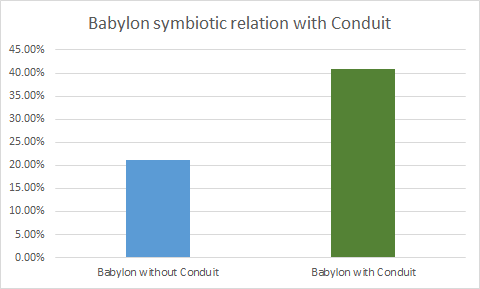
\includegraphics[scale=0.49]{figures/babylon_sym_conduit.png}
\caption{Babylon symbiotic relationship with Conduit}
\label{fig:babylon_sym_conduit}
\end{subfigure}
\begin{subfigure}[b]{0.49\textwidth}
	\centering
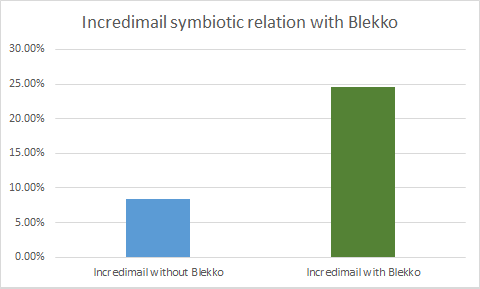
\includegraphics[scale=0.49]{figures/incredi_sym_blekko.png}
\caption{Incredimail symbiotic relationship with Blekko}
\label{fig:incredi_sym_blekko}
\end{subfigure}
\caption{Symbiotic relationship between companies}
	\label{fig:symbiotic_pagerank}
\end{figure}

\begin{figure}[h]
\centering
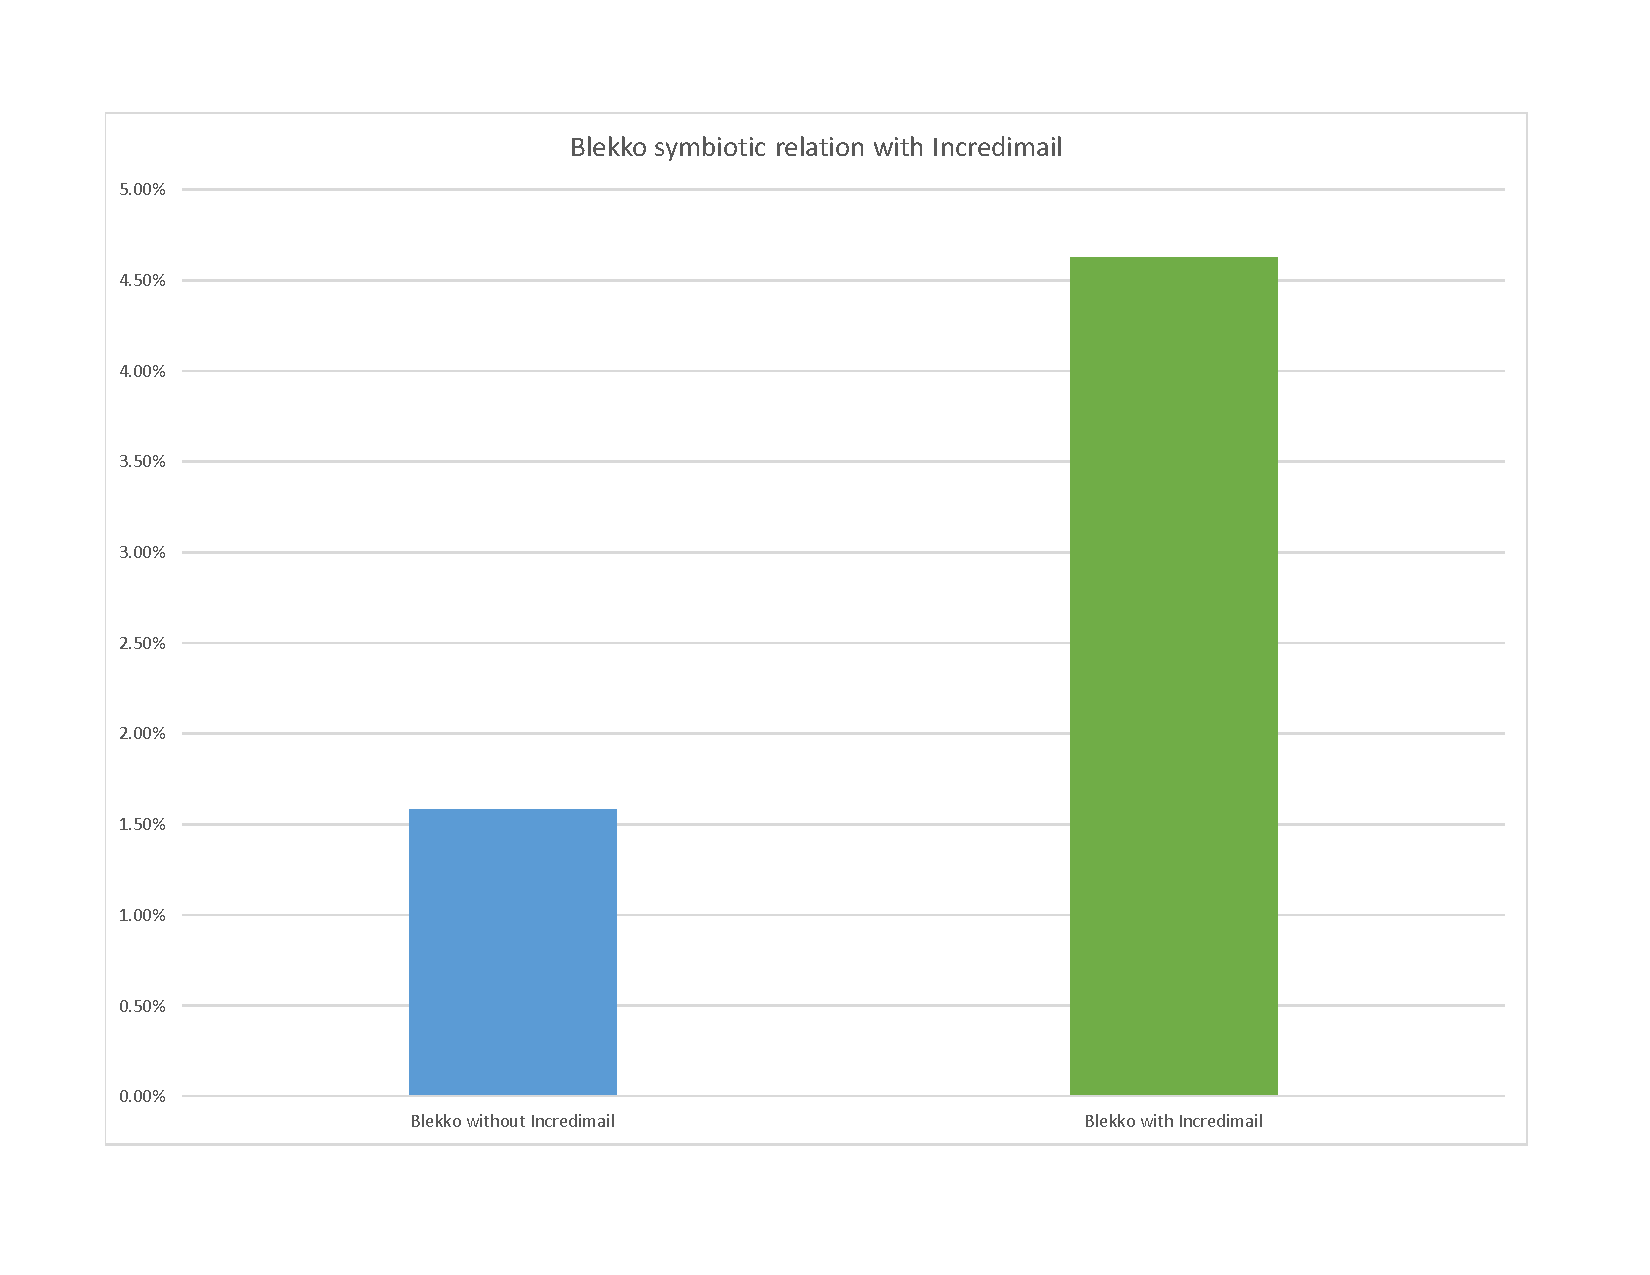
\includegraphics[width=\linewidth]{figures/blekko_sym_incredi.pdf}
\caption{Blekko symbiotic relationship with Incredimail}
\label{fig:blekko_sym_incredi}
\end{figure}


It is known that some company addons are getting to a user machine when they are "bundled" with add-ons of other companies. For example, the Ask Toolbars are integrated with the Java download\footnote{\url{https://java.com/en/download/faq/ask_toolbar.xml}}. During the installation of Java, users are presented with an option of downloading an Ask Toolbar, see \autoref{fig:ask_offer}.
\begin{figure}[h]
\centering
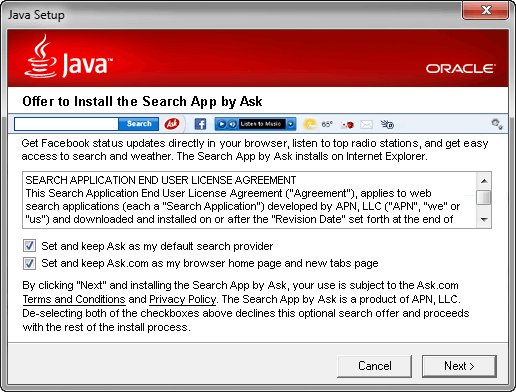
\includegraphics[scale=.8,angle=0]{figures/ask_offer.png}
\caption{Bundled ASK Toolbar installation}
\label{fig:ask_offer}
\end{figure}


\subsection{Clash Relationships}
\label{sec:clash_relations}

In \autoref{sec:symb_relations}, we have investigated symbiotic relationships between addon species, i.e. when one species benefit from another. Here, we will look for the opposite kind of relationship, it can be referred Parasitism, i.e. where one species benefits and causes harm to the other species, but we are referring to this relation as a clash between two (or more) species. The idea that lays in the way of of identifying clash relation is very similar to the way described in \autoref{sec:symb_relations}, again we are looking at the aggregated company scores, but this time we are looking for a company which score is getting lower when other company is present. In \autoref{fig:clash_pagerank}, you can see two examples for this relationship. The \autoref{fig:avira_clash_imesh} shows that when AntiVirus company Avira is present in ecosystem it causes an iMesh company to perform worth than in regular ecosystem. The same is shown in \autoref{fig:conduit_clash_hotspot}, between Conduit and Hotspot Shield company.

\begin{figure}[h]
\centering
\begin{subfigure}[b]{0.49\textwidth}
	\centering
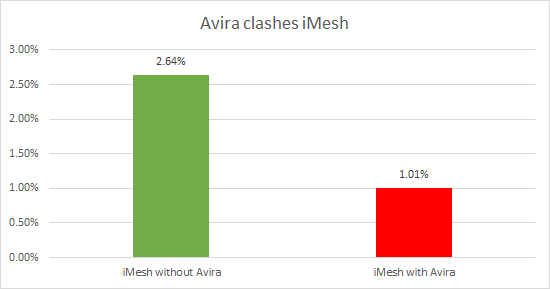
\includegraphics[scale=0.49]{figures/clashAviraImesh.png}
\caption{Avira clash relationship with iMesh}
\label{fig:avira_clash_imesh}
\end{subfigure}
\begin{subfigure}[b]{0.49\textwidth}
	\centering
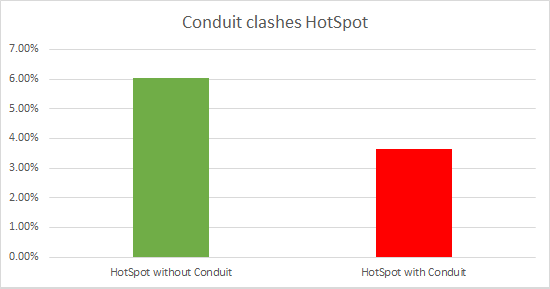
\includegraphics[scale=0.49]{figures/clashConduitHotSpot.png}
\caption{Conduit clash relationship with HotSpot}
\label{fig:conduit_clash_hotspot}
\end{subfigure}
\caption{Clash relationship between companies}
	\label{fig:clash_pagerank}
\end{figure}

Interesting validation for these measures could be applied if we would know about actual clash between companies from the \autoref{table:pagerank_scores} list. Having AntiVirus companies at the list comes handy, it is known that in most case two AV software programs can not exist on the same computer. Thus, using our terminology, the AV companies should have a clash relationship. And indeed, as shown in \autoref{fig:clash_av}, our algorithm detects AV companies as clashing.

\begin{figure}[h]
\centering
\begin{subfigure}[b]{0.49\textwidth}
	\centering
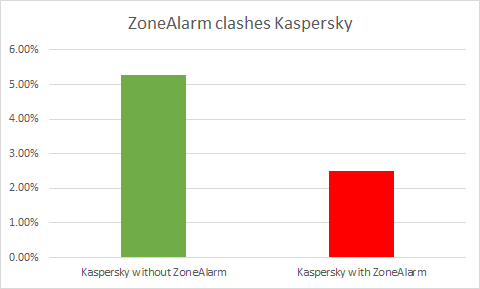
\includegraphics[scale=0.49]{figures/zone_clash_kaspersky.png}
\caption{ZoneAlarm clash relationship with Kaspersky}
\label{fig:zone_clash_kaspersky}
\end{subfigure}
\begin{subfigure}[b]{0.49\textwidth}
	\centering
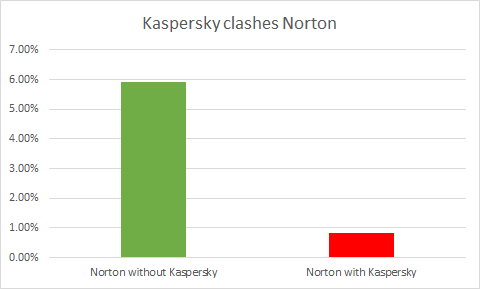
\includegraphics[scale=0.49]{figures/kaspersky_clash_norton.png}
\caption{Kaspersky clash relationship with Norton}
\label{fig:kaspersky_clash_norton}
\end{subfigure}
\caption{Clash relationship between AntiVirus companies}
	\label{fig:clash_av}
\end{figure}

\iffalse
After aggregating all add-ons for each for every company we have looked for what have happened to other company add-ons when PPR origin is a specific company.
For example, we have looked at HotSpot company and the impact it has on other companies.\\
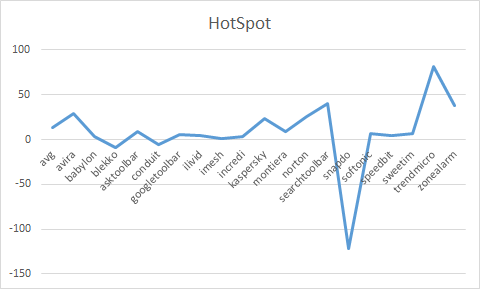
\includegraphics[scale=1.0]{hotspot.png}\\
As we can see from the chart some companies like trendmicro has a symbiosis with hotspot add-ons. While other companies, like SnapDo, are clashing with HotSpot add-ons.
This analysis, is even more interesting in light of recent security breach with Superfish and Komodia. After this security breach was identified, security researches where looking for more companies that have cooperated with Komodia. We believe that given that data, our algorithm would identify these companies as having a symbiosis with Komodia.
\fi

\iffalse
First, we needed some basic ranking of all add-ons from all companies, we believe that regular PageRank scores on this graph provide a good base line to all add-ons metrics. [Why do we need basic rankings? - RON][SELA] Basic ranking it is actually a baseline ranks, we were running a regular pagerank for this. It was used as a baseline, afterwards, for comparing how the rank of company addons has increased/decreased. BTW, this text is not in the thesis...
Then, we identified add-ons belonging to a company by looking for the company's name in addon descriptions. But what if the addon does not contain the company's name, can we still identify it as related to the company? To solve this problem, we applied an approach similar to the one we used to identify a "missing" addon. We ran PPR from all known add-ons of a specific company (for example, Babylon), and looked at all add-ons that drastically improved its rank compared to its previous rank given by PageRank.
By searching the addon names in the Web, many of them were found to be related to the company that originated the PPR (whose add-ons composed the PPR vector). For example,an  addon named tbmyba.dll, jumped from the 1200 rank position to the 15 rank position when running PPR from Babylon, and indeed we found that this addon is related to Babylon. 
After identifying all company add-ons, we decided to remove add-ons that are installed at fewer than 100 users' machines: these add-ons seemed to have almost no impact on the results but have made more difficult to look for tendencies between firms. [Why is that? - RON] [SELA] There were many addons that was installed only on few machines, we wanted to try to look at the addons "manually" and understand what is going on. Since the addons on small amount of machines did not have any impact, we could just remove them.\\
\fi


\section{Discussion}
We are comparing for each company its total weighted rank in PageRank with its total weighted rank in Personalized PageRank when another company is the PPR vector.
We have found that there are companies that co-exist well with other companies, there are even companies that improve greatly other companies add-ons rank.
We have also observed companies that cause other companies add-ons decline.



%\bibliographystyle{alpha}
\newpage
\appendix
\chapter{} 
\renewcommand{\figurename}{Appendix}

\begin{figure}[h]
\centering
\begin{subfigure}[b]{0.49\textwidth}
	\centering
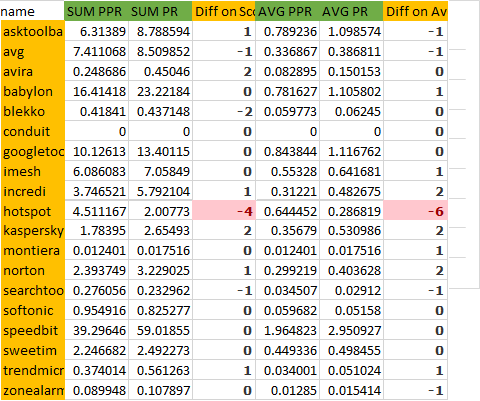
\includegraphics[scale=0.49]{figures/conduit_pr_scores.png}
\end{subfigure}
\begin{subfigure}[b]{0.49\textwidth}
	\centering
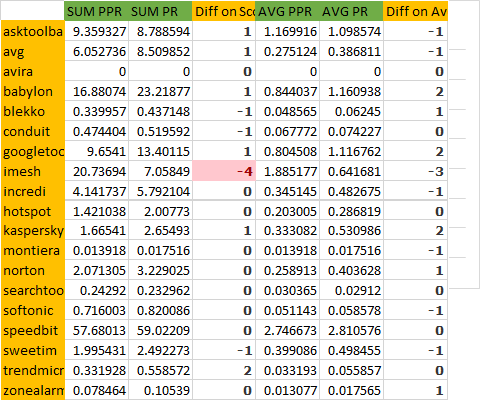
\includegraphics[scale=0.49]{figures/avira_pr_scores.png}
\end{subfigure}
\caption{PR scores}
	\label{fig:appendix_pr}
\end{figure}

\begin{figure}[h]
\centering
\begin{subfigure}[b]{0.49\textwidth}
	\centering
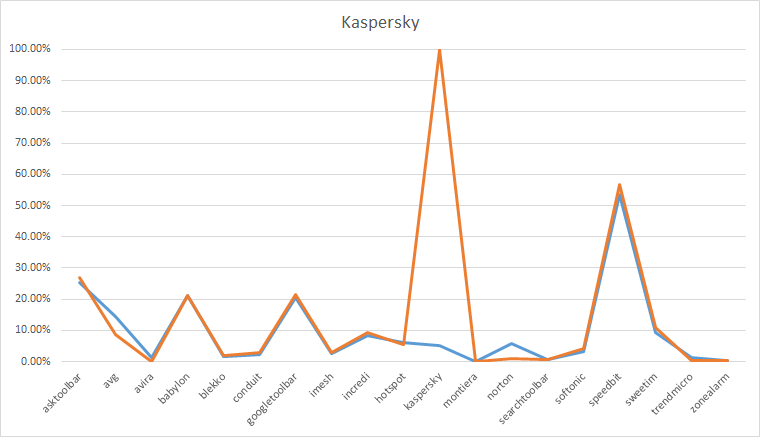
\includegraphics[scale=0.49]{figures/kaspersky_graph.png}
\end{subfigure}
\begin{subfigure}[b]{0.49\textwidth}
	\centering
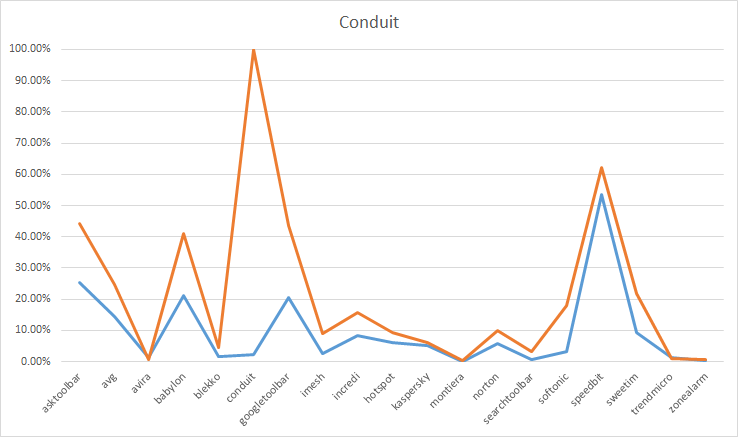
\includegraphics[scale=0.49]{figures/conduit_graph.png}
\end{subfigure}
\caption{Graph scores}
	\label{fig:appendix_pr}
\end{figure}

\begin{figure}[h]
\centering
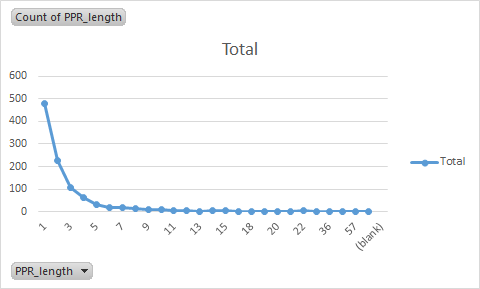
\includegraphics[scale=0.8]{figures/PPR_length_dist.png}
\caption{Personaliztion vector length}
\end{figure}



\bibliographystyle{apalike}
\bibliography{thesisdraft}
\addcontentsline{toc}{chapter}{Bibliography}

\end{document}

